% ju 14-5-22 01-N-Keywords-Thema.tex
\documentclass[a4paper,12pt,fleqn,parskip=half]{scrartcl}
\usepackage[ngerman]{babel}
\usepackage[utf8]{inputenc}
\usepackage[T1]{fontenc}

% Schrift
%\usepackage{lmodern}
\usepackage[osf,sc]{mathpazo} 
\usepackage[scale=.9,semibold]{sourcecodepro}   
\usepackage[osf]{sourcesanspro}  

\usepackage[headsepline]{scrlayer-scrpage}
\pagestyle{scrheadings}
\clearpairofpagestyles

\usepackage[table,dvipsnames,usenames]{xcolor}
\usepackage{textcase}
\usepackage{nameref}
\usepackage{hyperref}
\usepackage{tabularx}
\usepackage{multirow}
\usepackage{multicol}
\usepackage{caption, booktabs}
\usepackage{graphicx} 
\usepackage{scrhack}    
\usepackage{url}%% Links
\usepackage[inline]{enumitem}
\usepackage{pifont}
\usepackage{eurosym}% \euro 20,-
\usepackage{amsmath}
\usepackage{amsfonts}
\usepackage{amssymb}
\usepackage{array}            % Extending the array and tabular environments
\usepackage{chngcntr}         % Change the resetting of counters
\usepackage[version=4]{mhchem}
\usepackage{stmaryrd}
\usepackage{siunitx}
\usepackage{float}
\usepackage{csquotes}
\usepackage{subcaption}
\usepackage{mathtools}
\usepackage{icomma}%Dezimaltrennzeichen
\usepackage{multimedia}%Video: \movie[externalviewer]{(video.mov)}{video.mov}
\usepackage{epstopdf}
\usepackage{footnote}
\usepackage{qrcode}% Anwendung: \qrcode[hyperlink,level=Q,version=2,height=1cm]{\website}
\usepackage{underscore}% Unterstrich ____

% PDF Dokumente einbinden
\usepackage{pdfpages}% \includepdf[pages=-]{Tabellen/Excel.pdf}
\RequirePackage{lastpage}  % Pagecounter

\addto\captionsngerman{%
\renewcommand{\figurename}{Abb.}
\renewcommand{\tablename}{Tab.}
}

% listings
\usepackage{listings}
\lstset{basicstyle=\linespread{1}\ttfamily\small,floatplacement=!htb,captionpos=t,abovecaptionskip=.5\baselineskip,belowcaptionskip=.5\baselineskip,upquote=true,showstringspaces=false,inputencoding=utf8,tabsize=4,
    	keywordstyle=\bfseries ,
	commentstyle=\color{rot5},
	stringstyle=\color{orange},
	breaklines=true,
  	postbreak=\mbox{\textcolor{black}{$\hookrightarrow$}\space},
	breakatwhitespace=false
}
\lstset{literate={á}{{\'a}}1 {é}{{\'e}}1 {í}{{\'i}}1 {ó}{{\'o}}1 {ú}{{\'u}}1 {Á}{{\'A}}1 {É}{{\'E}}1 {Í}{{\'I}}1 {Ó}{{\'O}}1 {Ú}{{\'U}}1 {à}{{\`a}}1 {è}{{\`e}}1 {ì}{{\`i}}1 {ò}{{\`o}}1 {ù}{{\`u}}1 {À}{{\`A}}1 {È}{{\'E}}1 {Ì}{{\`I}}1 {Ò}{{\`O}}1 {Ù}{{\`U}}1 {ä}{{\"a}}1 {ë}{{\"e}}1 {ï}{{\"i}}1 {ö}{{\"o}}1 {ü}{{\"u}}1 {Ä}{{\"A}}1 {Ë}{{\"E}}1 {Ï}{{\"I}}1 {Ö}{{\"O}}1 {Ü}{{\"U}}1 {â}{{\^a}}1 {ê}{{\^e}}1 {î}{{\^i}}1 {ô}{{\^o}}1 {û}{{\^u}}1 {Â}{{\^A}}1 {Ê}{{\^E}}1 {Î}{{\^I}}1 {Ô}{{\^O}}1 {Û}{{\^U}}1 {œ}{{\oe}}1 {Œ}{{\OE}}1 {æ}{{\ae}}1 {Æ}{{\AE}}1 {ß}{{\ss}}1 {ű}{{\H{u}}}1 {Ű}{{\H{U}}}1 {ő}{{\H{o}}}1 {Ő}{{\H{O}}}1 {ç}{{\c c}}1 {Ç}{{\c C}}1 {ø}{{\o}}1 {å}{{\r a}}1 {Å}{{\r A}}1 {€}{{\EUR}}1 {£}{{\pounds}}1 {~}{{\textasciitilde}}1 {-}{{-}}1 }

% bibliography
\usepackage[
    bibencoding=utf8,
    backend=biber,% bibtex, biber
    backref=false,backrefstyle=three+,url=true,urldate=comp,abbreviate=false,maxnames=20
]{biblatex} %Paket laden
\DeclareBibliographyCategory{cited}
\let\defaultcite\cite\renewcommand*\cite[2][]{\addtocategory{cited}{#2}\defaultcite[#1]{#2}}
\let\defaulttextcite\textcite\renewcommand*\textcite[2][]{\addtocategory{cited}{#2}\defaulttextcite[#1]{#2}}
\setcounter{biburllcpenalty}{7000}
\setcounter{biburlucpenalty}{8000}
\AfterPackage{biblatex}{
	\PreventPackageFromLoading[\errmessage{Sie haben versucht, das Cite-Paket zu laden, das nicht mit biblatex kompatibel ist.}]{cite}
}

\hypersetup{%
	%pdftitle={\titel},
	%pdfsubject={Latex},
	%pdfauthor={\autor},
	%pdfcreator={\autor}, 
	bookmarksnumbered=true,
	breaklinks=true,
	%colorlinks=true,	   
	linkcolor=rot5,		
	filecolor=blau5,		
	urlcolor=blau5,			
	citecolor=ForestGreen
}

\linespread{1.1}
\setlist{itemsep=0pt}
\widowpenalty10000
\clubpenalty10000
\tolerance1000   

\usepackage[left=2cm,right=2cm,top=1cm,bottom=1cm,includeheadfoot]{geometry}
%\usepackage[left=4cm,right=2cm,top=1cm, bottom=1cm,includeheadfoot]{geometry}
%\usepackage[left=6cm,right=1cm,top=1cm, bottom=1cm,includeheadfoot]{geometry}
%\usepackage[landscape=true,left=2cm,right=2cm,top=1cm,bottom=1cm,includeheadfoot]{geometry}%quer

% eigene Farbe definieren
% Adobe Prozessfarben: CMYK: 100,50,0,35 -> 1,0.5,0,0.35
\definecolor{orange}{cmyk}{0,0.55,0.61,0}   % 0,55,61,0
\definecolor{blau5}{cmyk}{1,0.77,0.1,0.01}  % 100,77,10,
\definecolor{rot5}{cmyk}{0.22,1,1,0.19}     % 22,100,100,19
\definecolor{grau2}{cmyk}{0,0,0,0.1}        % 0,0,0,40
\definecolor{blau}{cmyk}{0.93,0.66,0,0.21}% 

% Literatur
\bibliography{content/literatur}
\bibliography{content/literatur-kfz}
\bibliography{content/literatur-sport}

%%%%%%%%%%%%%%%%%%%%%%%%%%%%%%%%%%%%%%%%%%%%%%%%%%%%%%%
\newcommand{\name}{Jan Unger}% anpassen!!!!!
\newcommand{\thema}{Thema}% anpassen!!!!!
\newcommand{\quelle}{\name}
\newcommand{\website}{https://bw-ju.de/}
\newcommand{\github}{https://github.com/ju1-eu}
%%%%%%%%%%%%%%%%%%%%%%%%%%%%%%%%%%%%%%%%%%%%%%%%%%%%%%%

\ihead{\textbf{Quelle:} \quelle}%{Kopfzeile innen}
\ohead{\textbf{Datum:} \today}  %{Kopfzeile außen}
\ifoot{\textbf{Thema:} \thema}  %{Fußzeile  innen}
\ofoot{Seite {\thepage} von {\pageref{LastPage}}}%{Fußzeile  außen}

\title{\thema}
\author{\name}
\date{\today}

\begin{document}
	%\thispagestyle{empty}
	%\maketitle
	%\newpage
	%\setcounter{page}{1}

	%%%%%%%%%%%%%%%%%%%%%%%%%%%%%%%%%%%%%%%%%%%
	\begin{center}
		\textbf{\Large \thema}\\%14pt
		\vspace{0.8em}
		%\datum	
		\qrcode[hyperlink,level=Q,version=2,height=1cm]{\website}
		%\qrcode[hyperlink,level=Q,version=2,height=1cm]{\github}
	\end{center}
	%%%%%%%%%%%%%%%%%%%%%%%%%%%%%%%%%%%%%%%%%%%

	\subsection*{Keywords}%\label{sec:Deadline}\index{Deadline}
	% Checkliste
	\begin{itemize}[label=\checkmark] %\itemsep -2pt
		\item Begriff 
	\end{itemize}


	%ju 13-Mai-22 01-Keywords-Thema.tex
\section{Keywords - Thema}\label{keywords-thema}

	Tabellenbuch (\textcite{bell:2021:tabellenbuchKfz} S. 281)

	\emph{Website} \footnote{\url{\website}} 	
	
	Arbeitszeitermittlung (\autoref{fig:Arbeitszeitermittlung}).
	\begin{figure}[!h]% hier: !hb
		\centering
		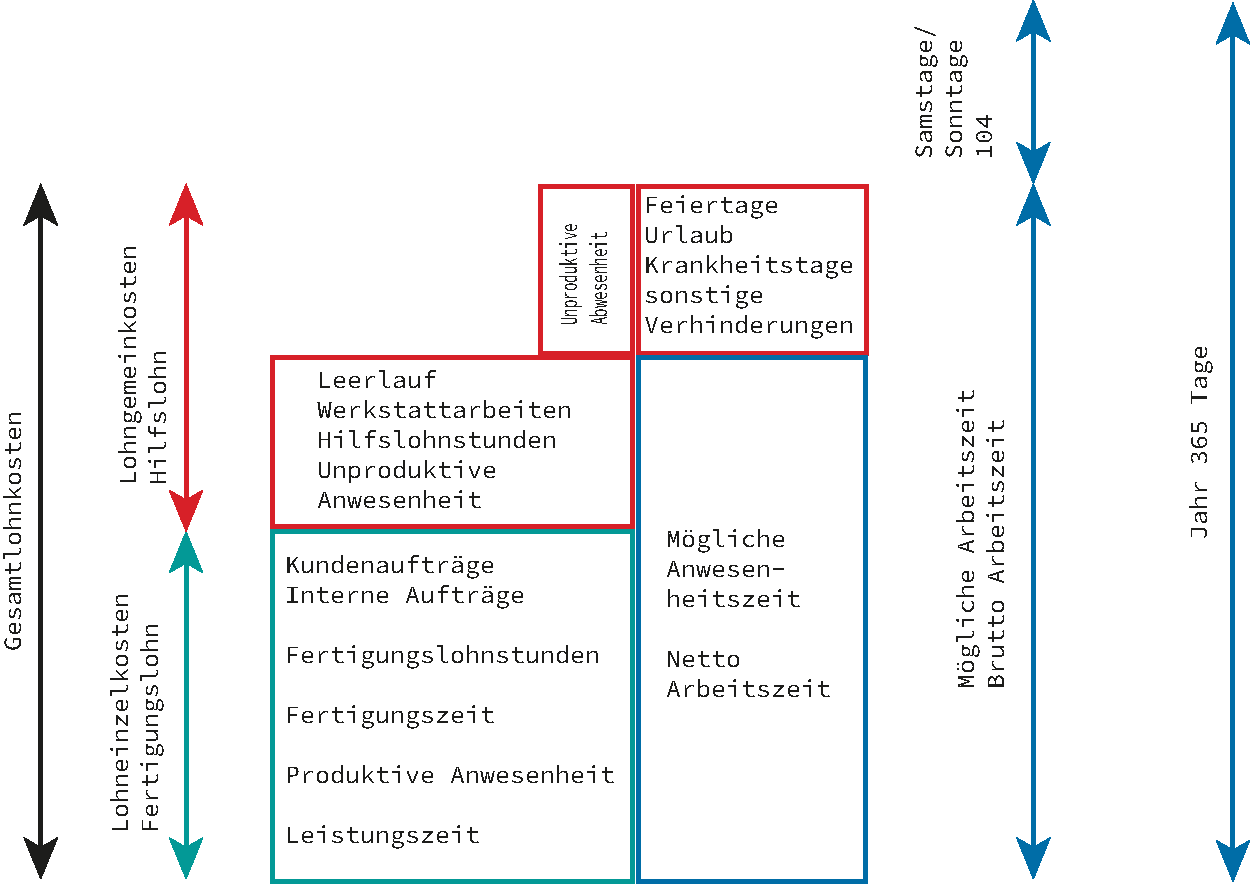
\includegraphics[width=.75\textwidth]{images/Skizze/Arbeitszeitermittlung.pdf}
		\caption{Arbeitszeitermittlung}\label{fig:Arbeitszeitermittlung}%% anpassen
	\end{figure}
	
	%% ju 15-5-2022 input-PDFs.txt 

\chapter{Rechenbeispiele}% book, print anpassen

% -------
\section{Umsatzerlöse}\label{sec:01-Umsatzerloese}\index{01-Umsatzerloese}
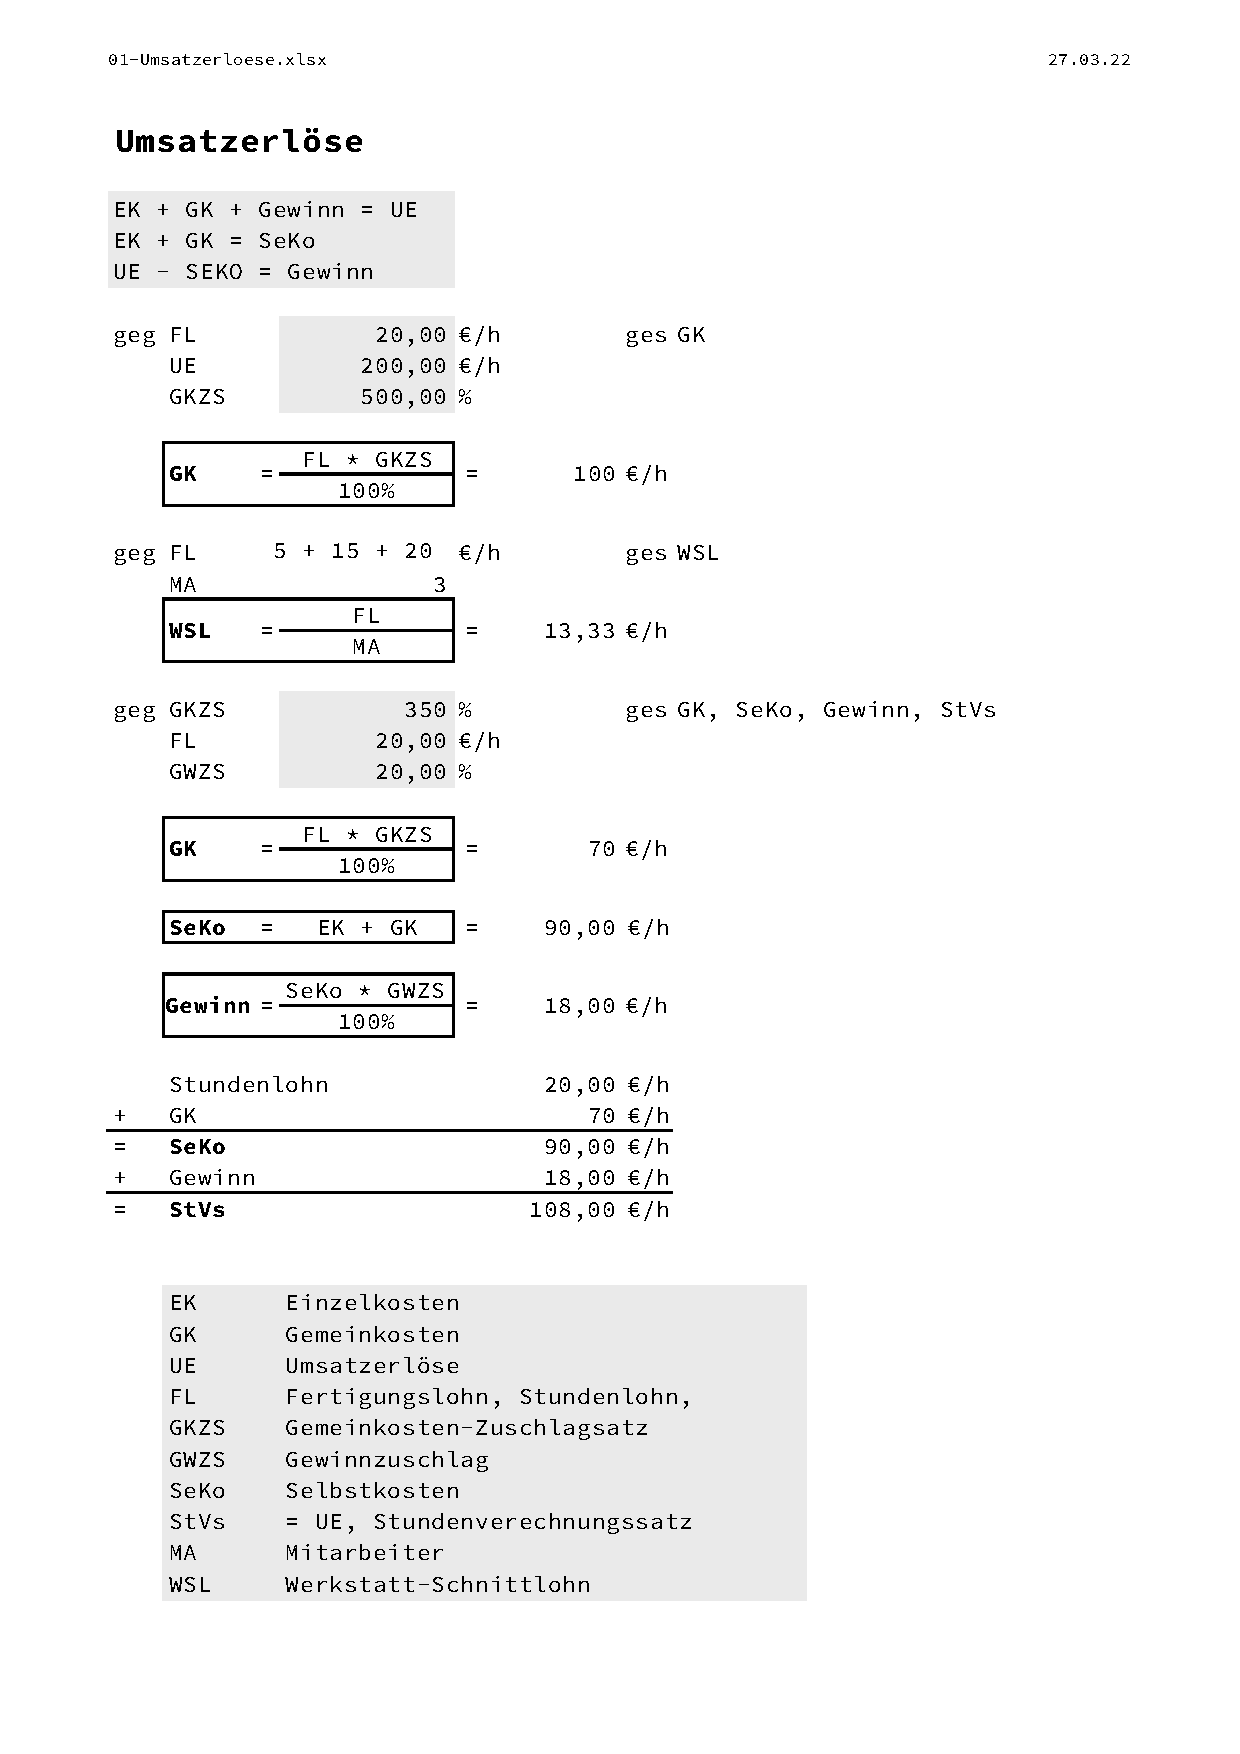
\includepdf[pages=-]{Tabellen/PDF/01-Umsatzerloese.pdf}

% -------
\section{AT-Steuer}\label{sec:02-AT-Steuer}\index{02-AT-Steuer}
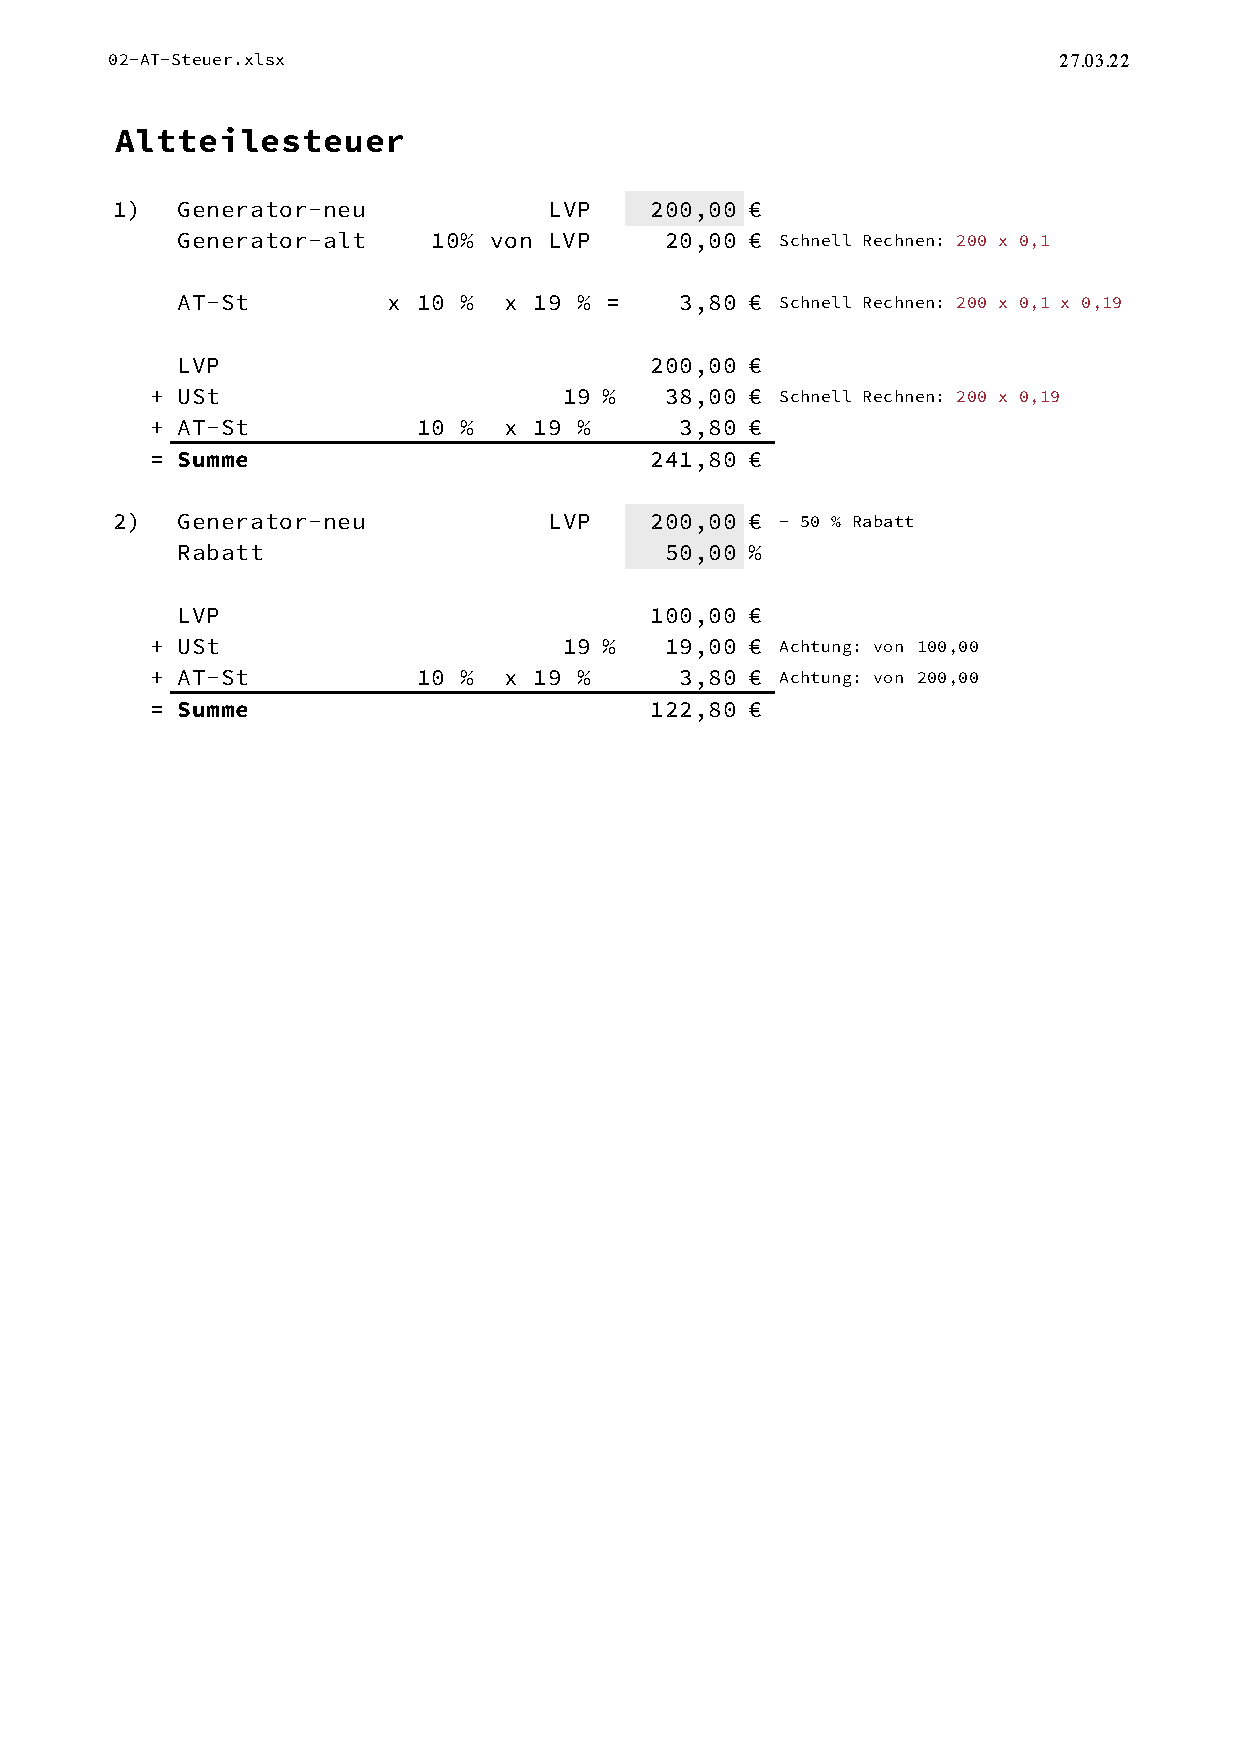
\includepdf[pages=-]{Tabellen/PDF/02-AT-Steuer.pdf}

% -------
\section{Ersatzteilpreiskalkulation}\label{sec:03-Ersatzteilpreiskalkulation}\index{03-Ersatzteilpreiskalkulation}
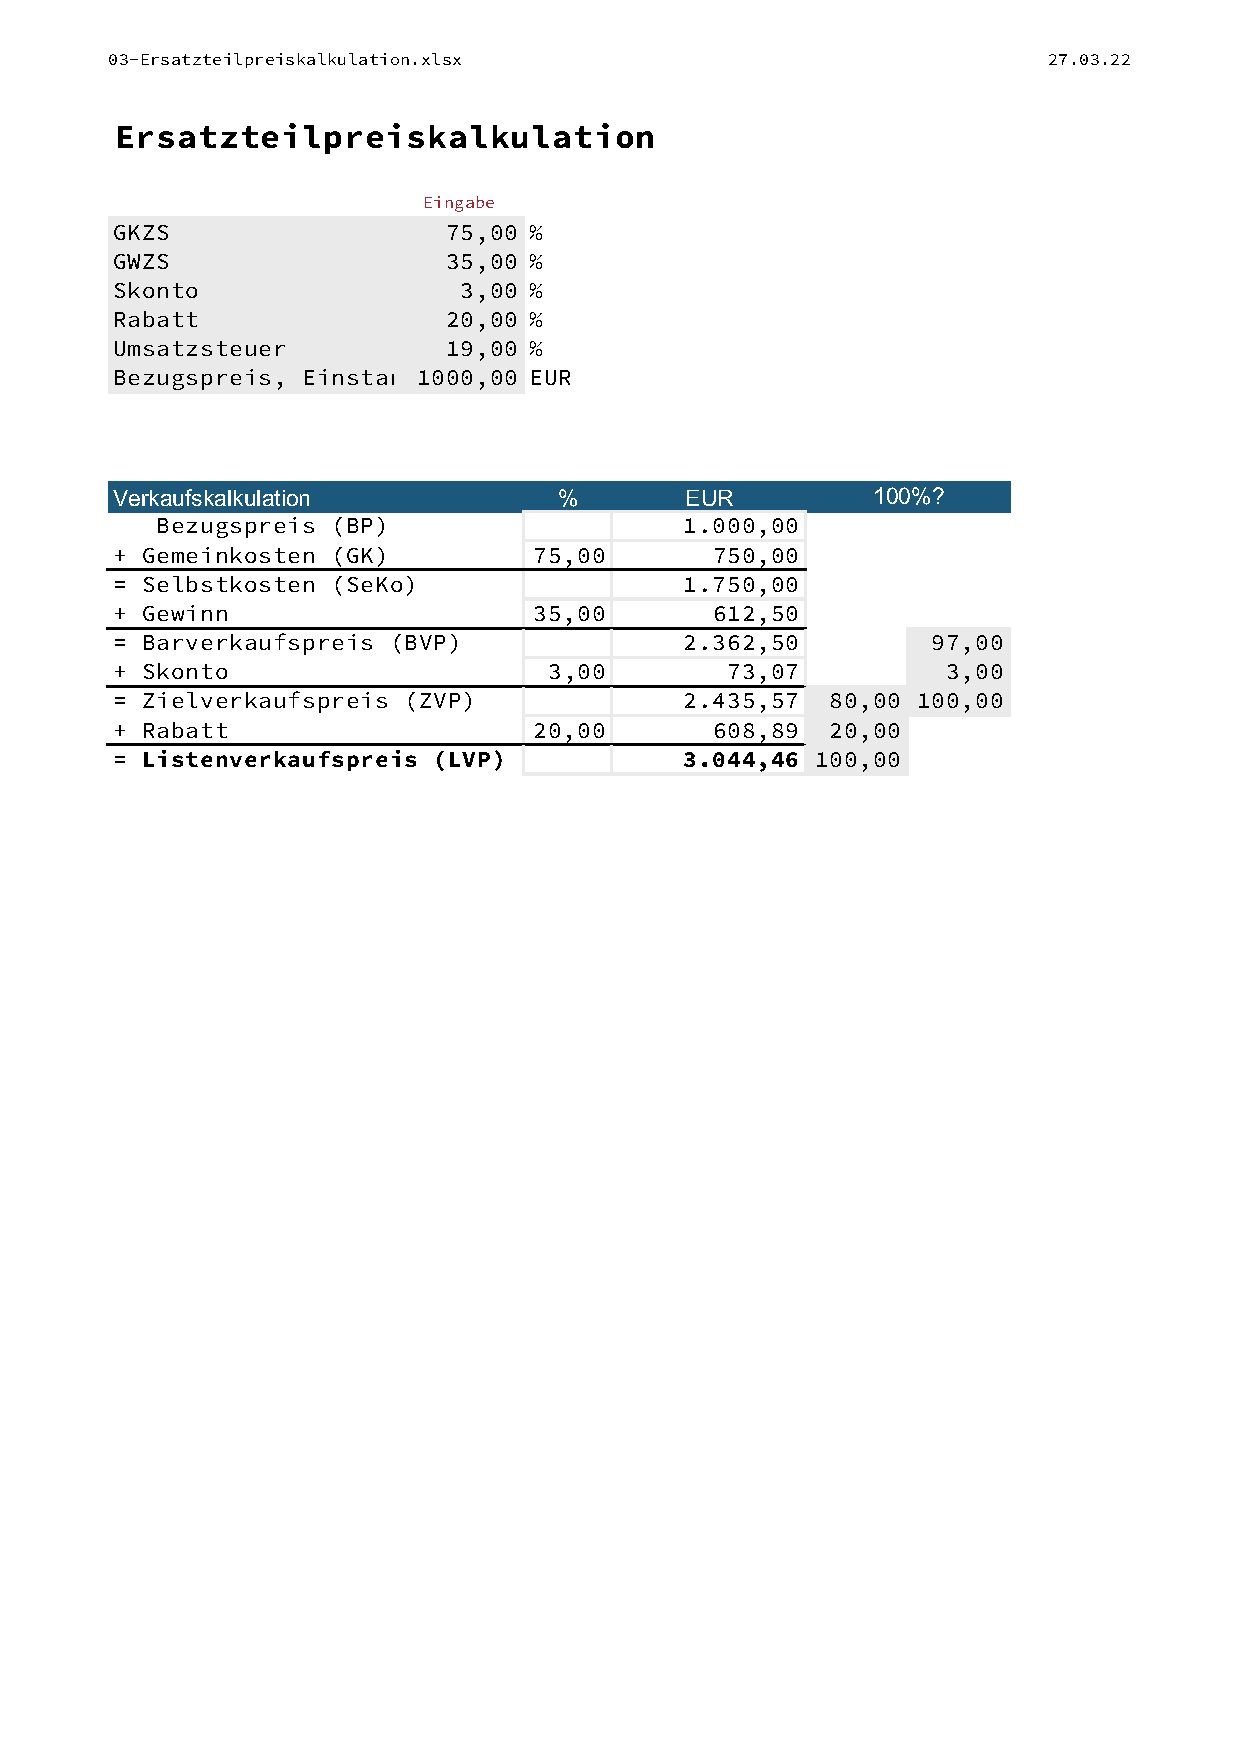
\includepdf[pages=-]{Tabellen/PDF/03-Ersatzteilpreiskalkulation.pdf}




\chapter{Übungsaufgaben}

% -------
\section{U01 - Ersatzteilpreiskalkulation - KI - HSP - KF}\label{sec:U01-Ersatzteilpreiskalkulation-KI-HSP-KF}\index{U01-Ersatzteilpreiskalkulation-KI-HSP-KF}
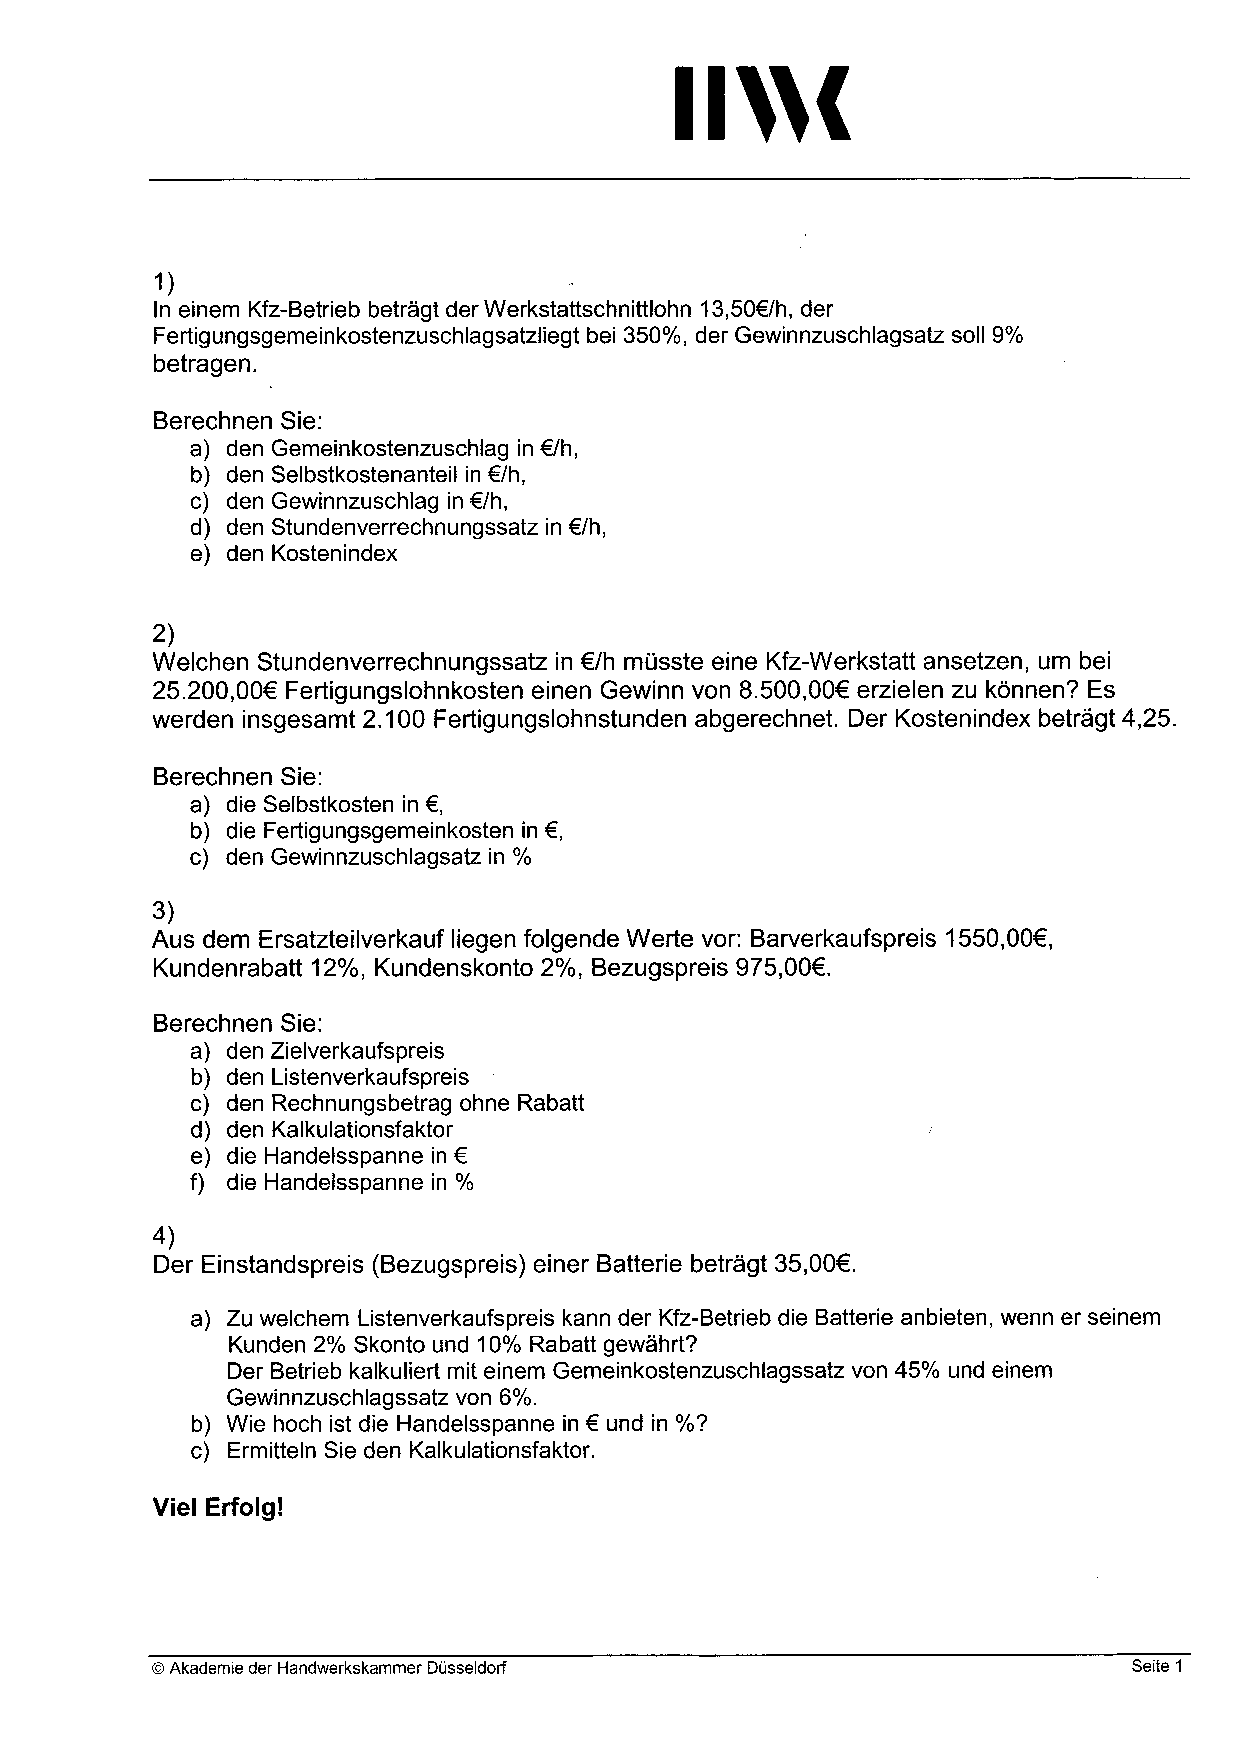
\includepdf[pages=-]{Tabellen/PDF/U01-Ersatzteilpreiskalkulation-KI-HSP-KF.pdf}
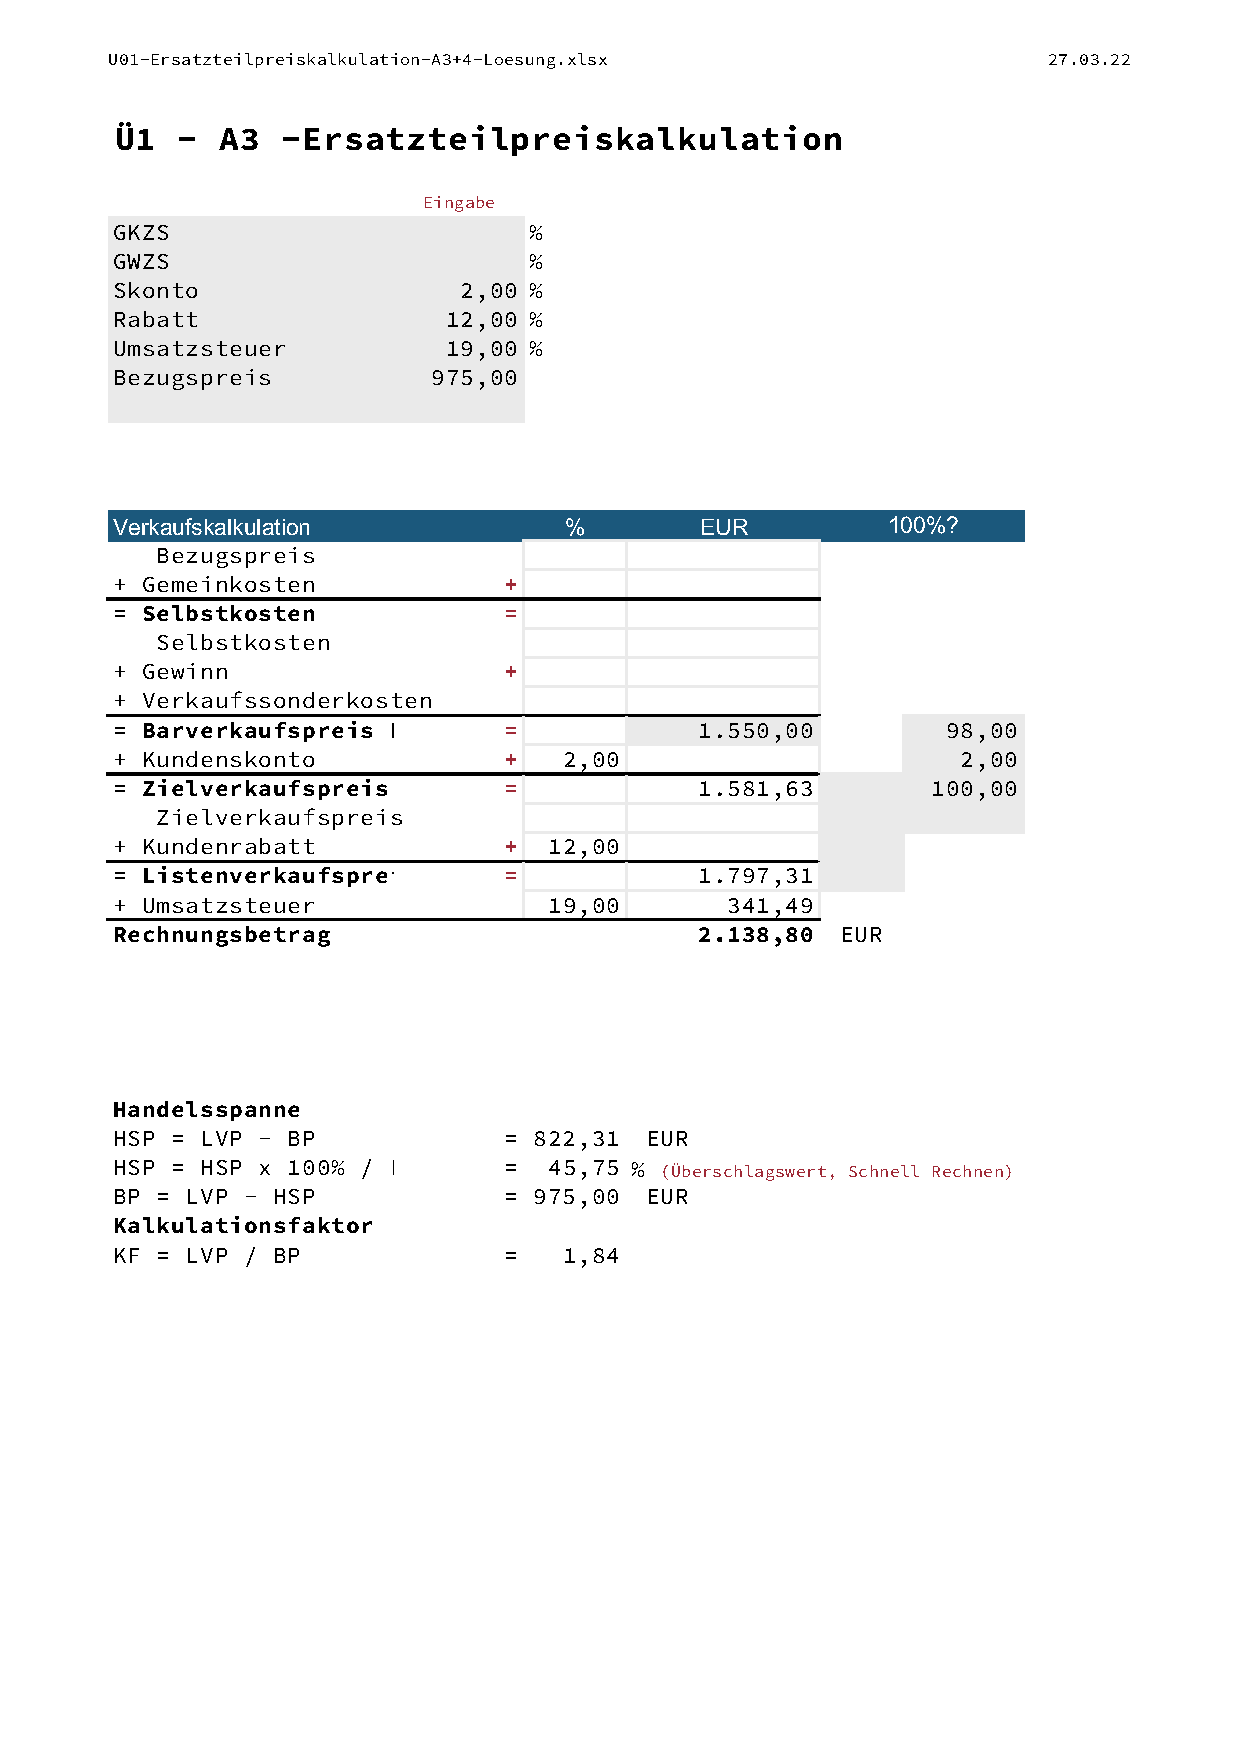
\includepdf[pages=-]{Tabellen/PDF/U01-Ersatzteilpreiskalkulation-A3+4-Loesung.pdf}

% -------
\section{U02 - StVs - WI - KI - Kostenvoranschlag}\label{sec:U02-StVs-WI-KI-Kostenvoranschlag}\index{U02-StVs-WI-KI-Kostenvoranschlag}
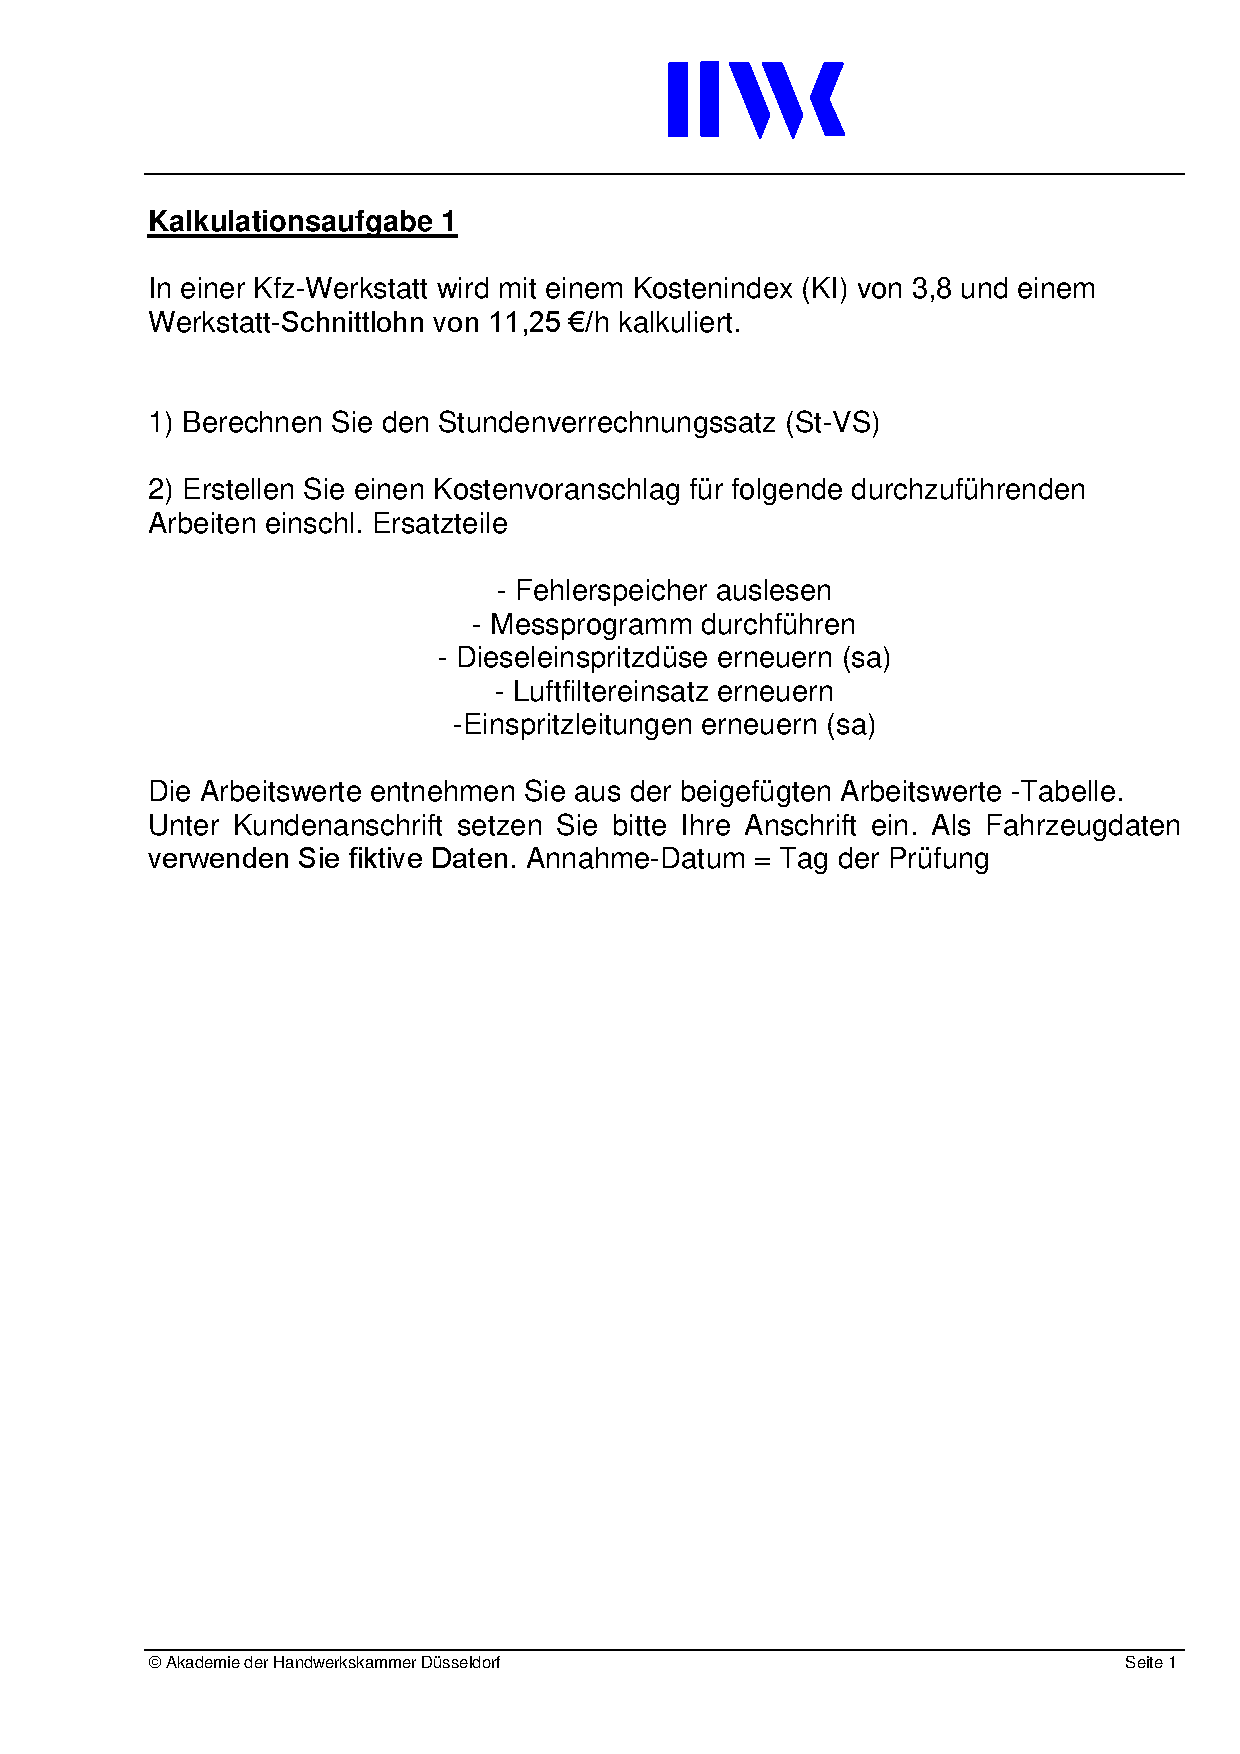
\includepdf[pages=-]{Tabellen/PDF/U02-StVs-WI-KI-Kostenvoranschlag.pdf}
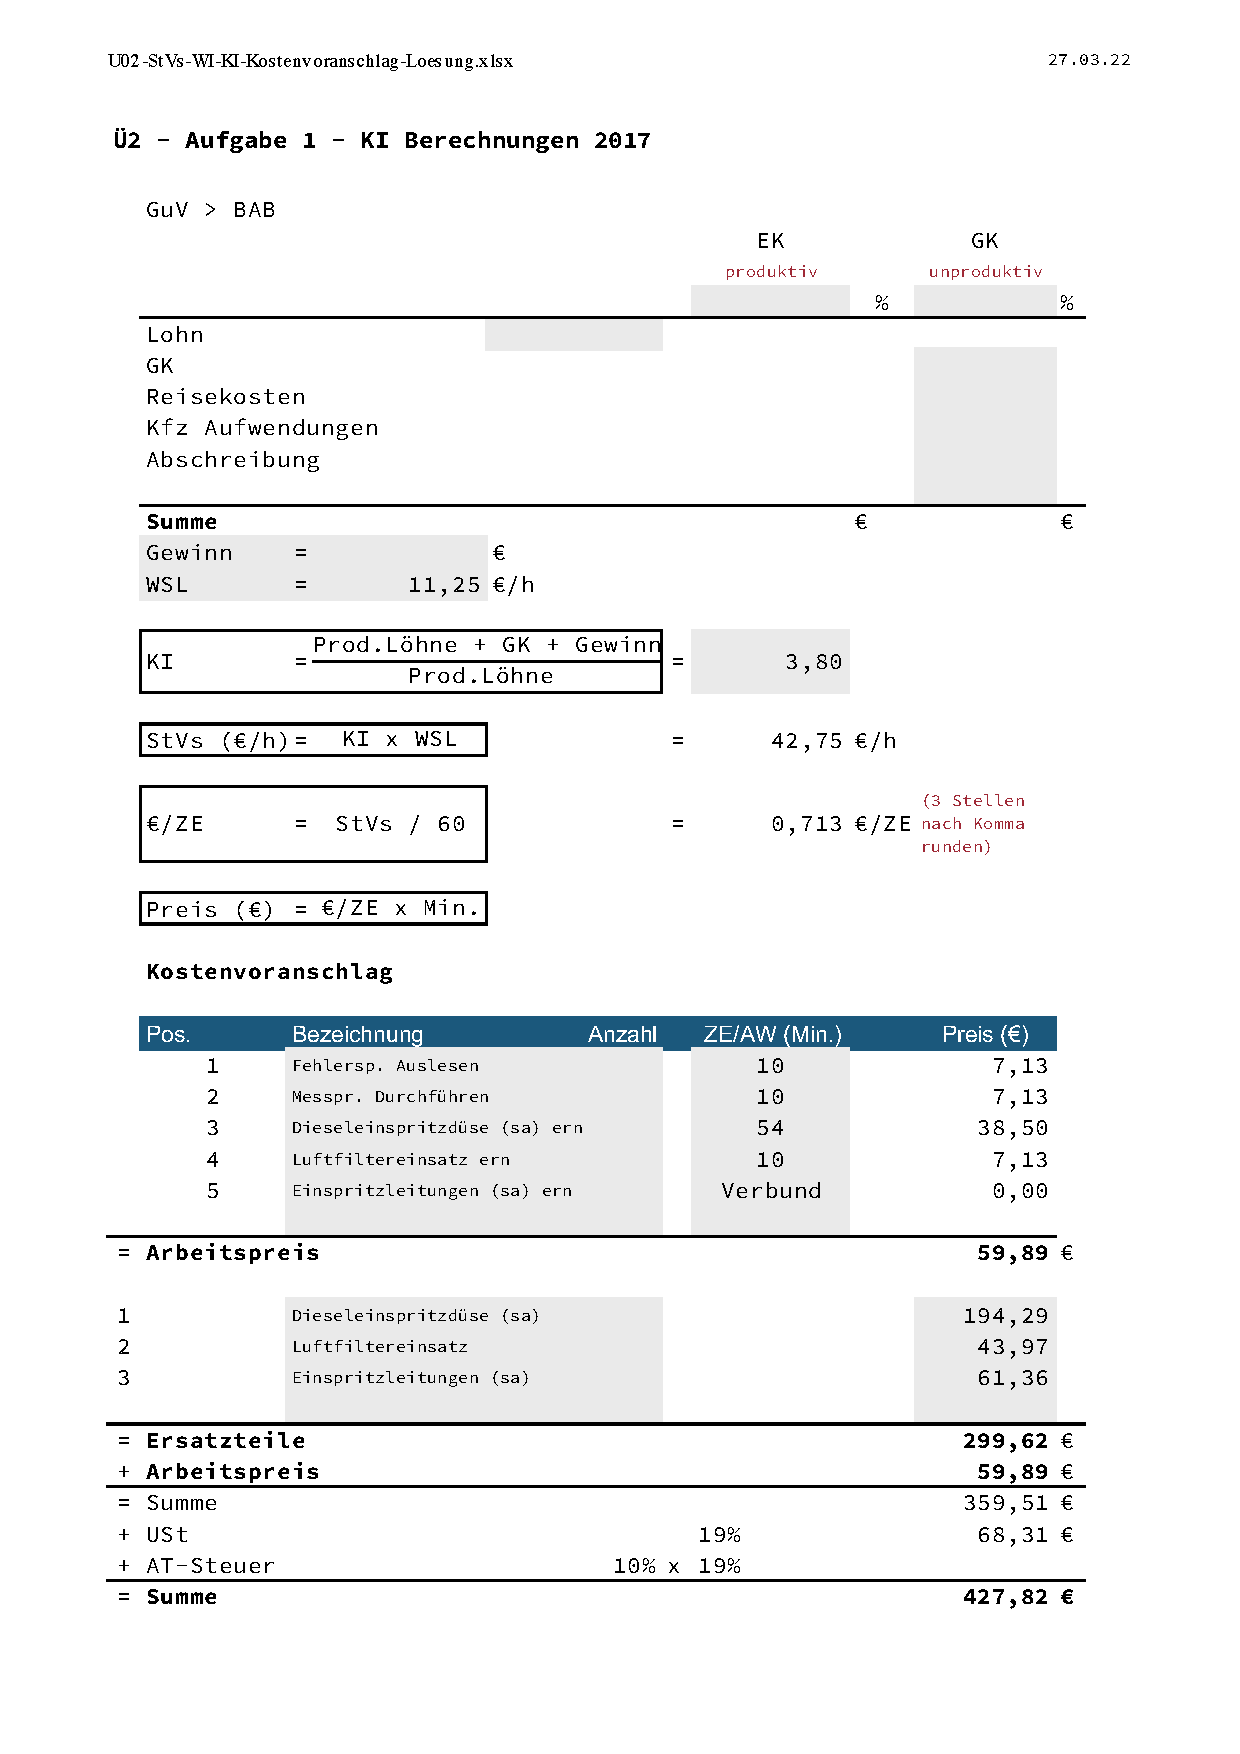
\includepdf[pages=-]{Tabellen/PDF/U02-StVs-WI-KI-Kostenvoranschlag-Loesung.pdf}

% -------
\section{U03 - Kundenrechnung - Kostenvoranschlag - AW-Vs - UR - WI}\label{sec:U03-Kundenrechnung-Kostenvoranschlag-AW-Vs-UR-WI}\index{U03-Kundenrechnung-Kostenvoranschlag-AW-Vs-UR-WI}
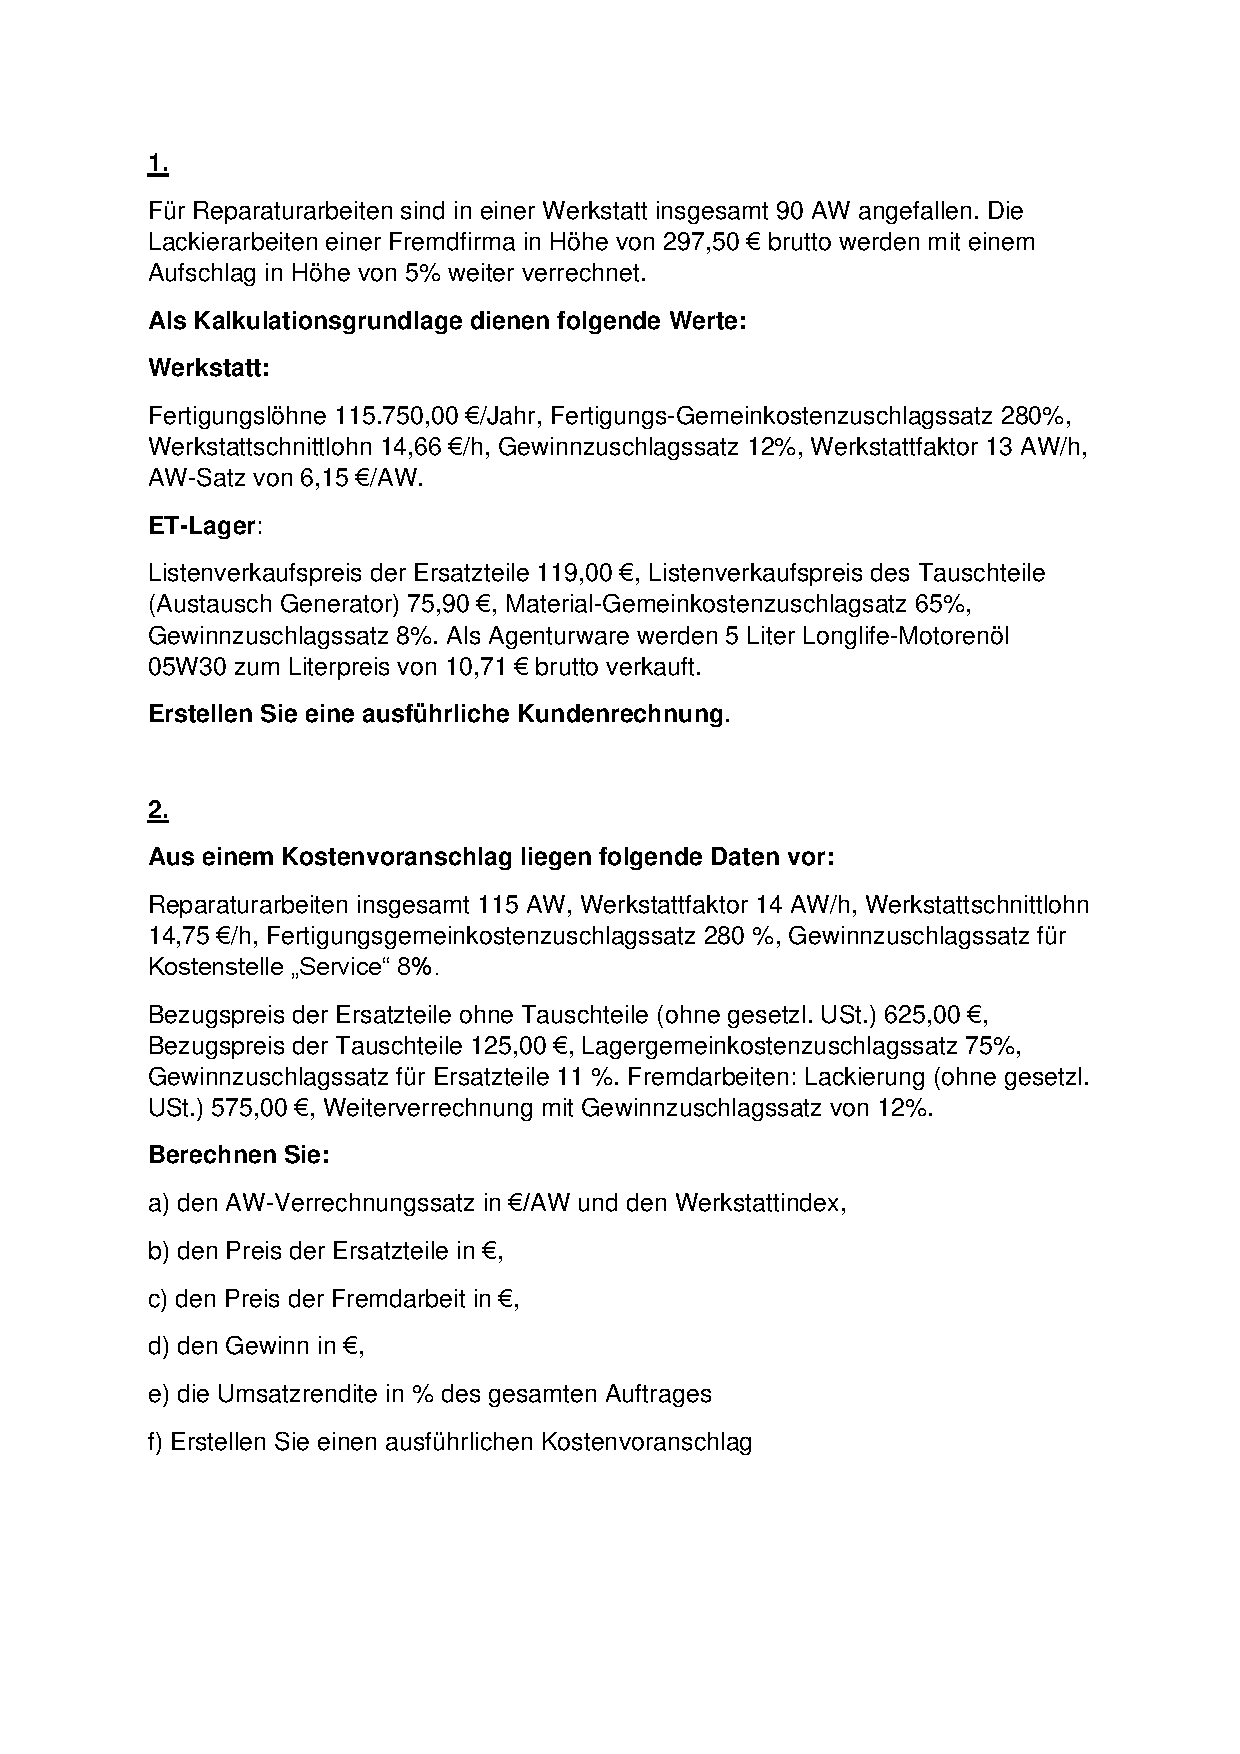
\includepdf[pages=-]{Tabellen/PDF/U03-Kundenrechnung-Kostenvoranschlag-AW-Vs-UR-WI.pdf}}
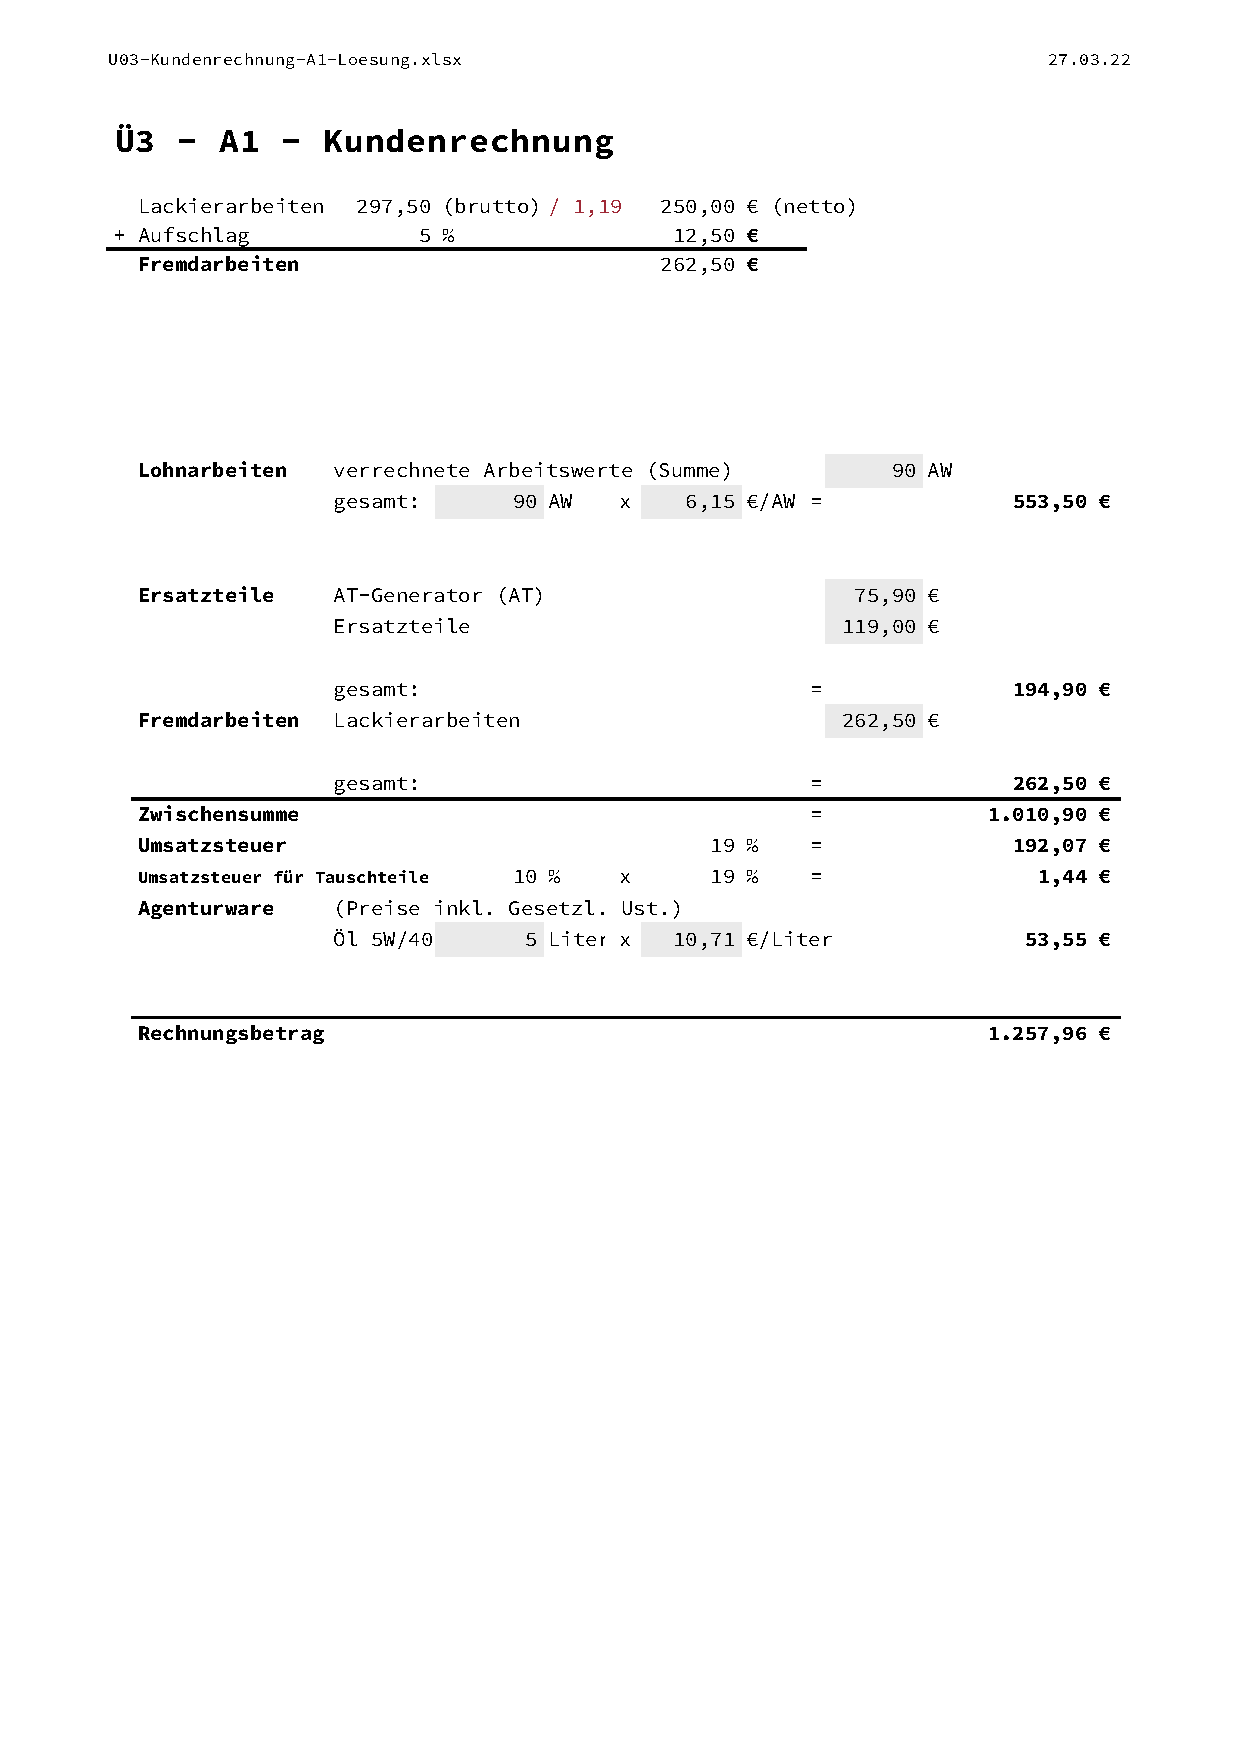
\includepdf[pages=-]{Tabellen/PDF/U03-Kundenrechnung-A1-Loesung.pdf}

% -------
\section{U04 - Werkstattabrechnung - Arbeitszeit - A1 - 4 von 10}\label{sec:U04-Werkstattabrechnung-Arbeitszeit_1-4_von10}\index{U04-Werkstattabrechnung-Arbeitszeit_1-4_von10}
\includepdf[pages=-]{Tabellen/PDF/U04-Werkstattabrechnung-Arbeitszeit_1-4_von10.pdf}

% -------
\section{U05 - Gesamtarbeitszeit - StVs - AW-Vs - Flh}\label{sec:U05-Gesamtarbeitszeit-StVs-AW-Vs-Flh}\index{U05-Gesamtarbeitszeit-StVs-AW-Vs-Flh}
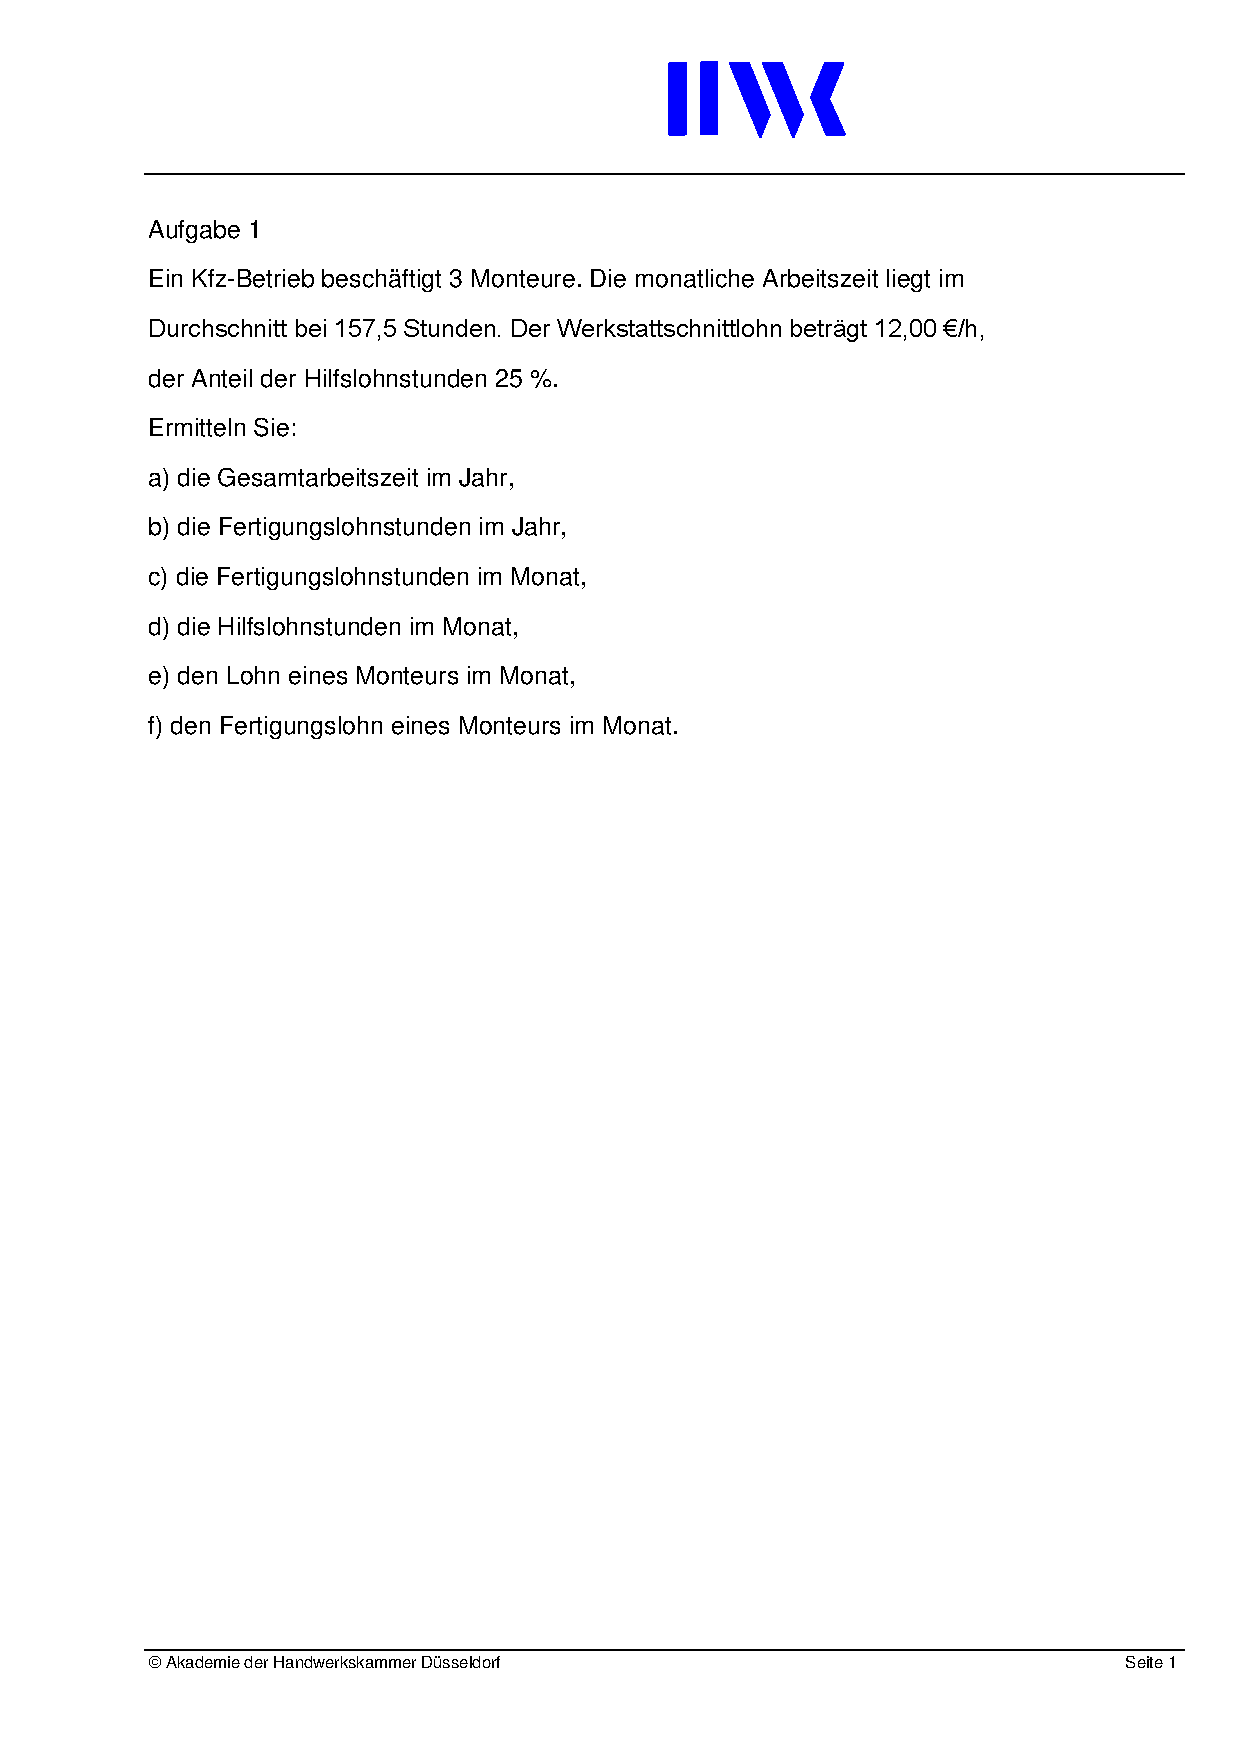
\includepdf[pages=-]{Tabellen/PDF/U05-Gesamtarbeitszeit-StVs-AW-Vs-Flh.pdf}

% -------
\section{U06 - Situationsaufgabe - Fritz}\label{sec:U06-Situationsaufgabe-Fritz-Loesung}\index{U06-Situationsaufgabe-Fritz-Loesung}
%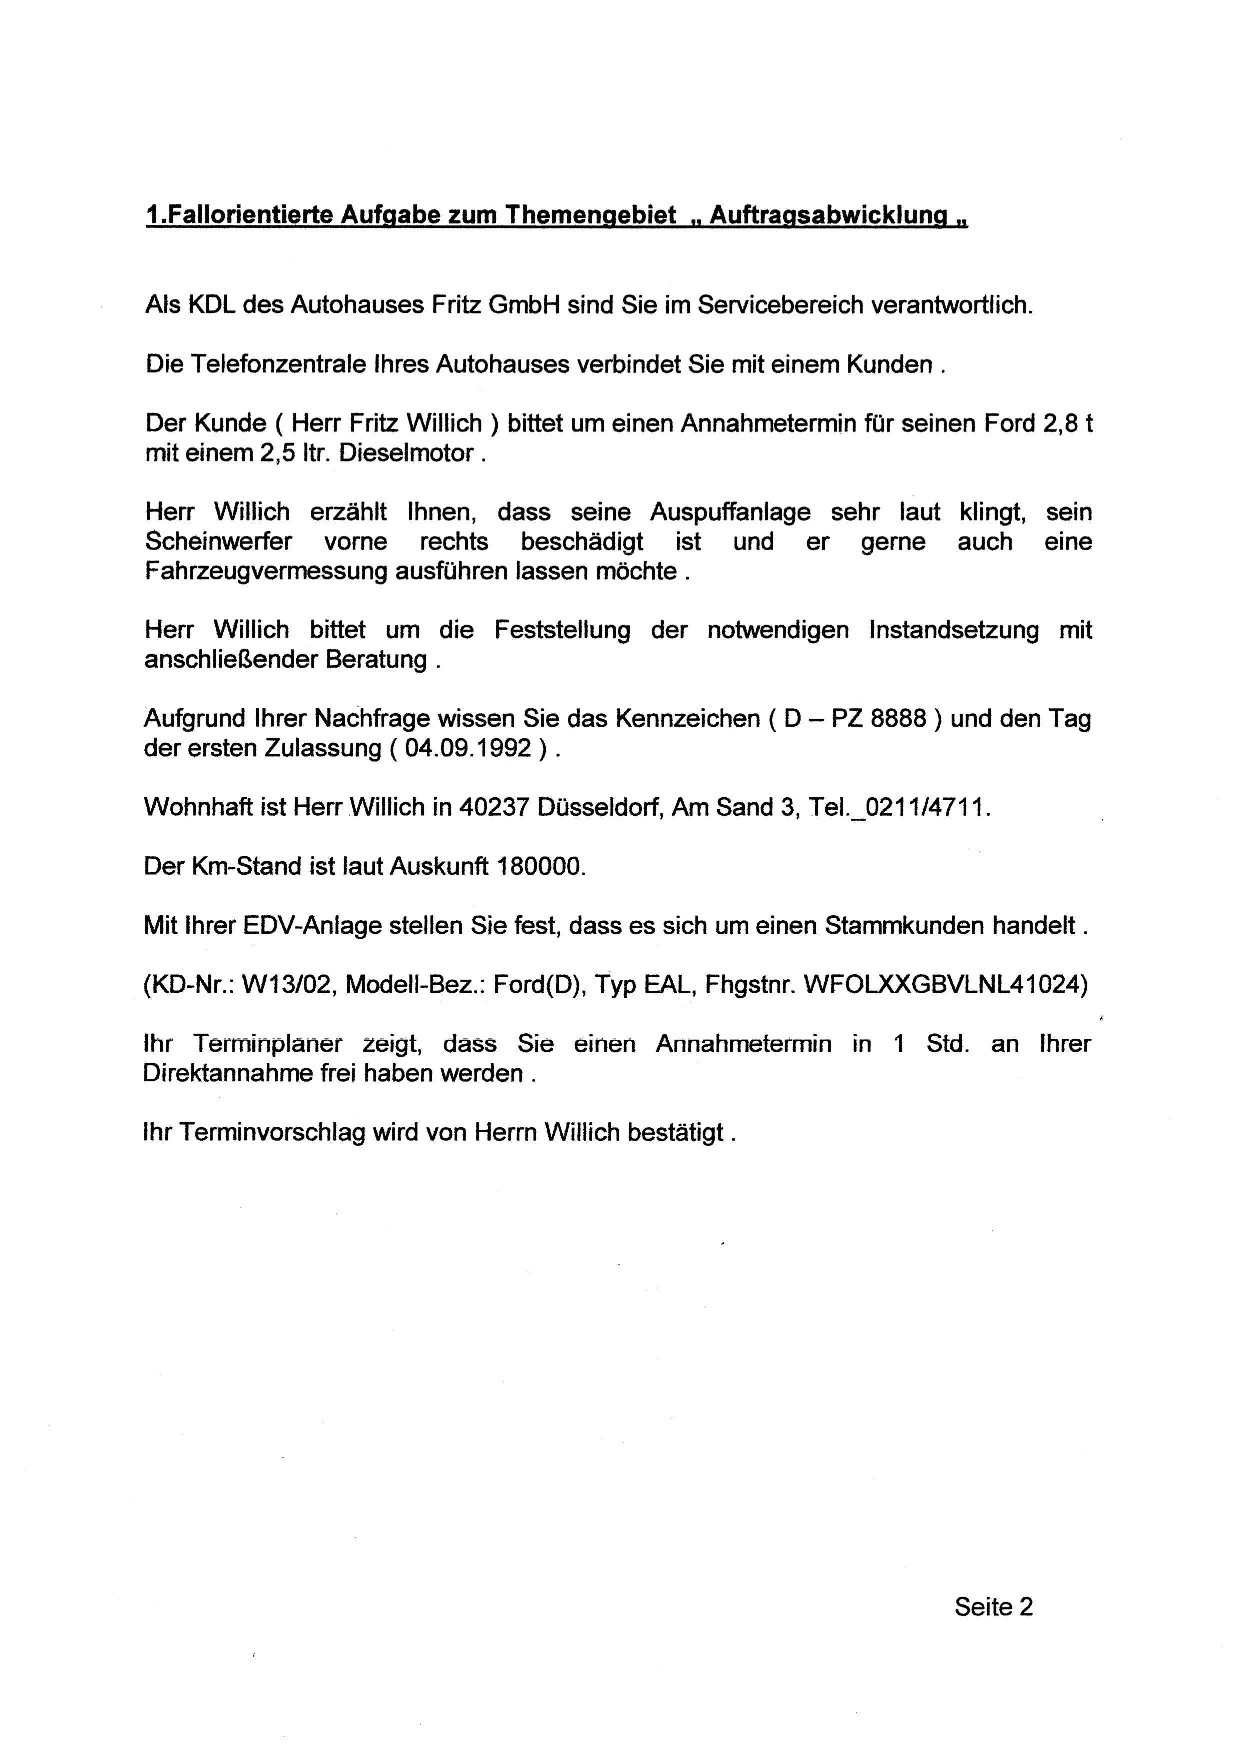
\includepdf[pages=-]{Tabellen/PDF/U06-Situationsaufgabe-Fritz-Loesung.pdf}
%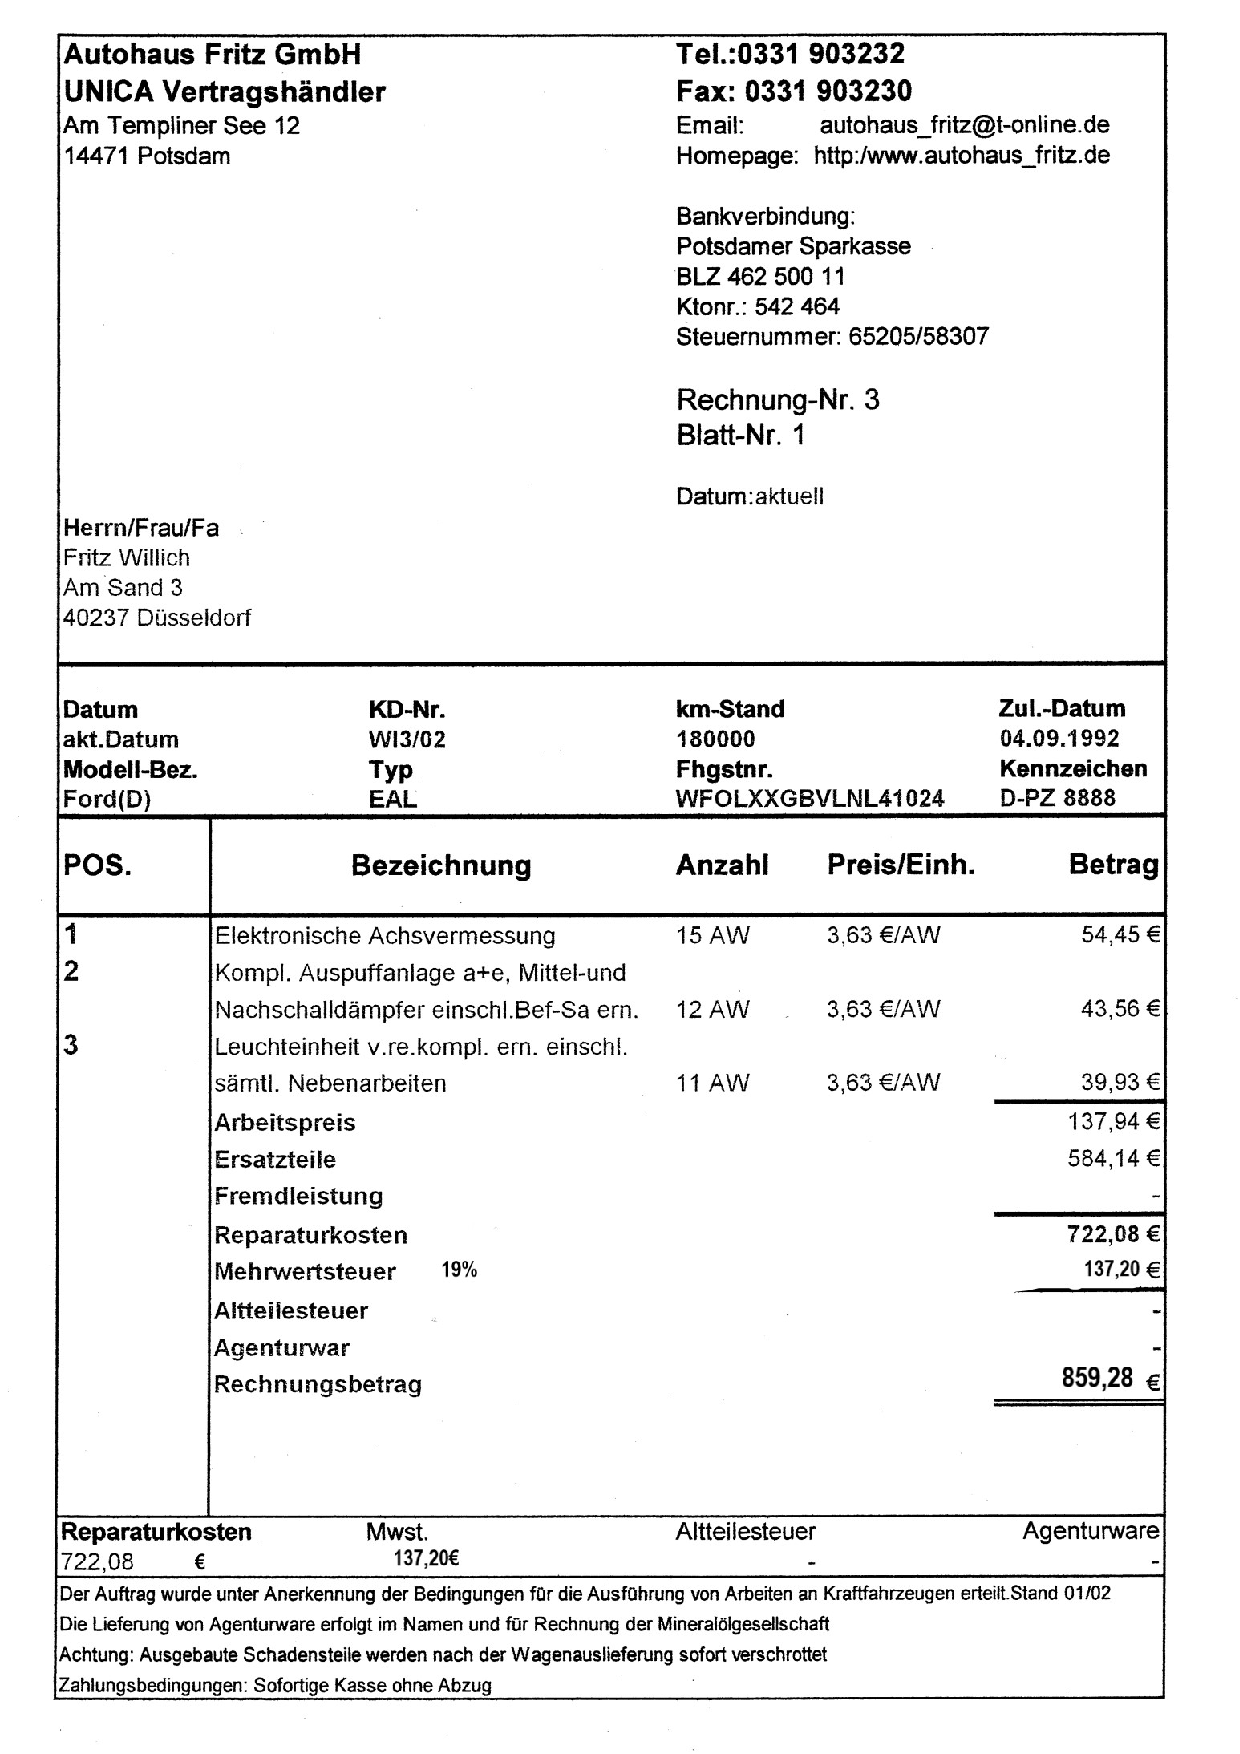
\includepdf[pages=-]{Tabellen/PDF/U06-Situationsaufgabe-Fritz-Rechnung.pdf}
%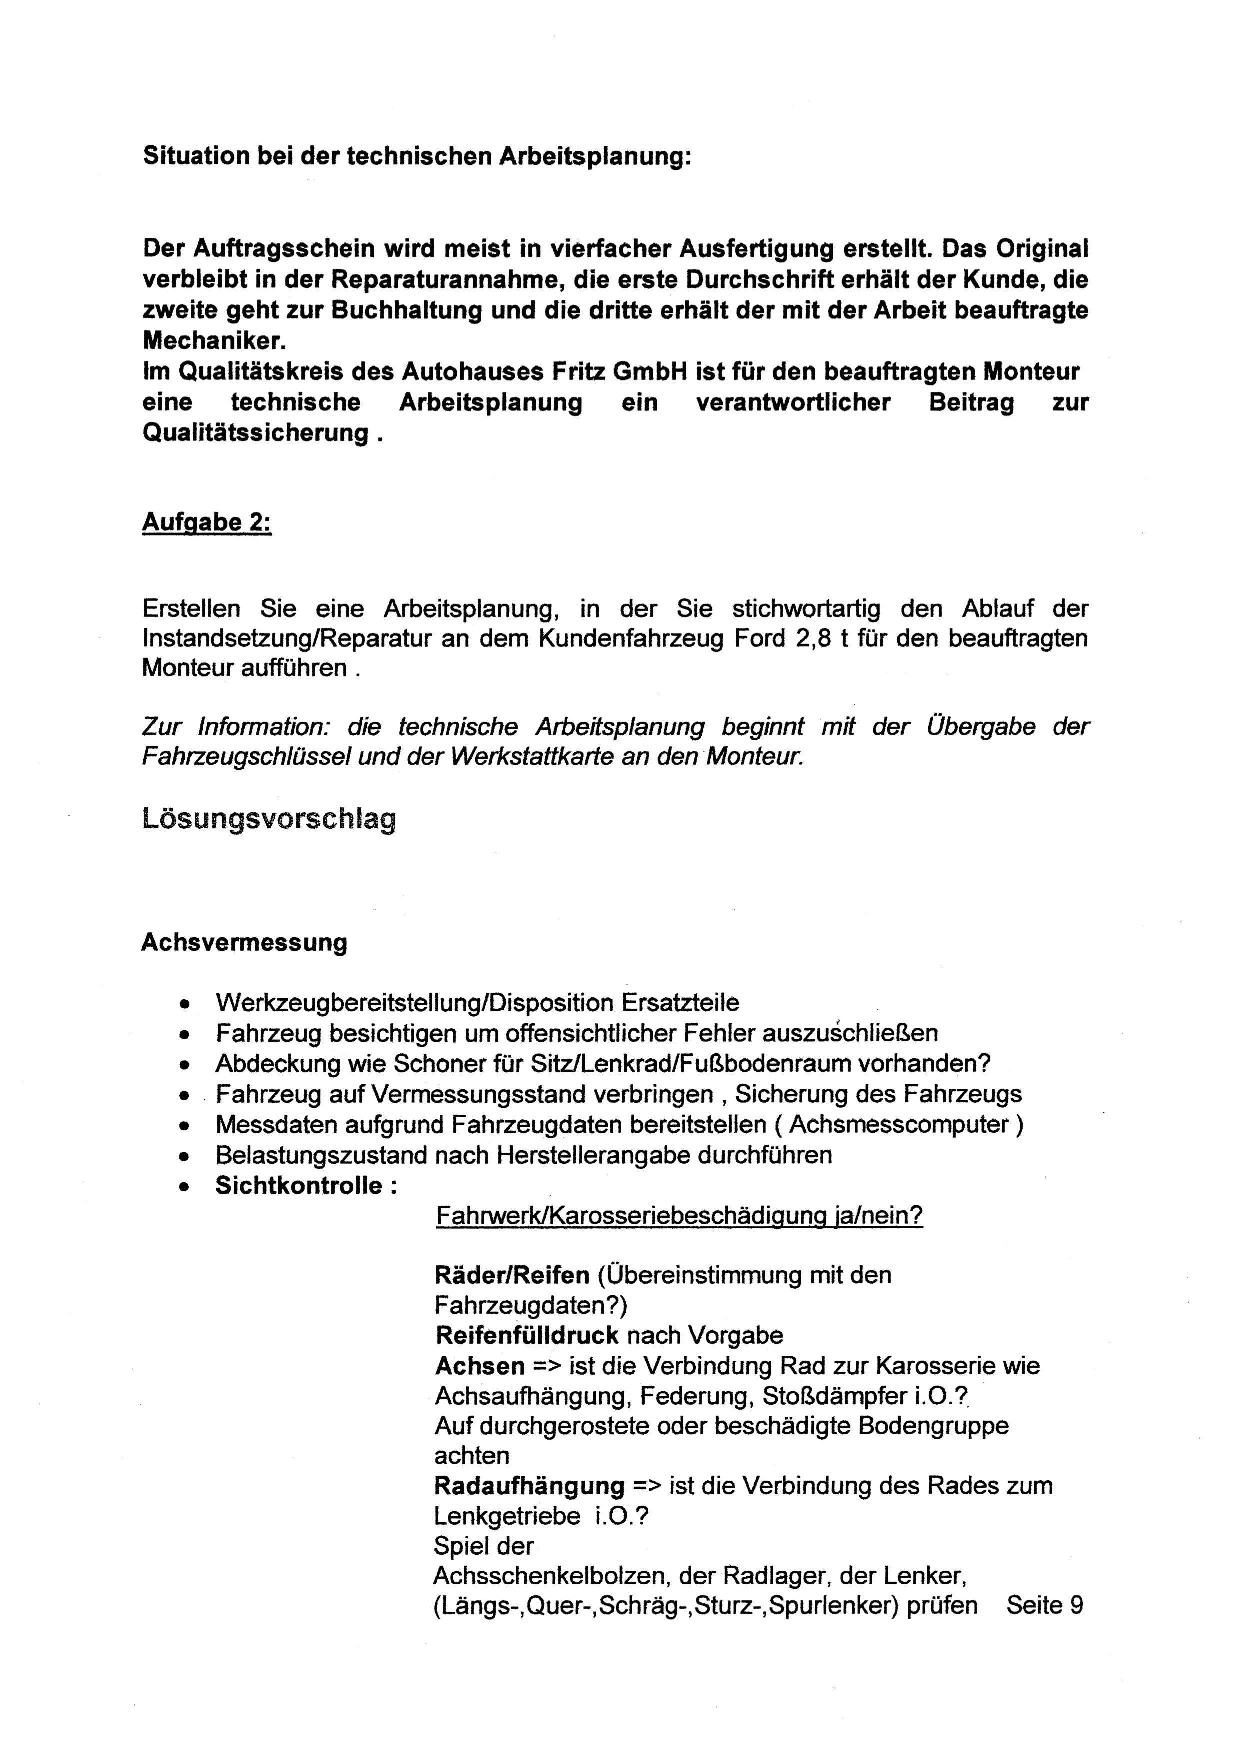
\includepdf[pages=-]{Tabellen/PDF/U06-Situationsaufgabe-Fritz-Arbeitsplanung.pdf}


% -------
\section{U07 - Aufgabe - KV1 - Stauscheibenpoti - AT}\label{sec:U07-Aufgabe-KV1-Stauscheibenpoti-AT}\index{U07-Aufgabe-KV1-Stauscheibenpoti-AT}

\includepdf[pages=-]{Tabellen/PDF/U07-Aufgabe-KV1-Stauscheibenpoti-AT.pdf}
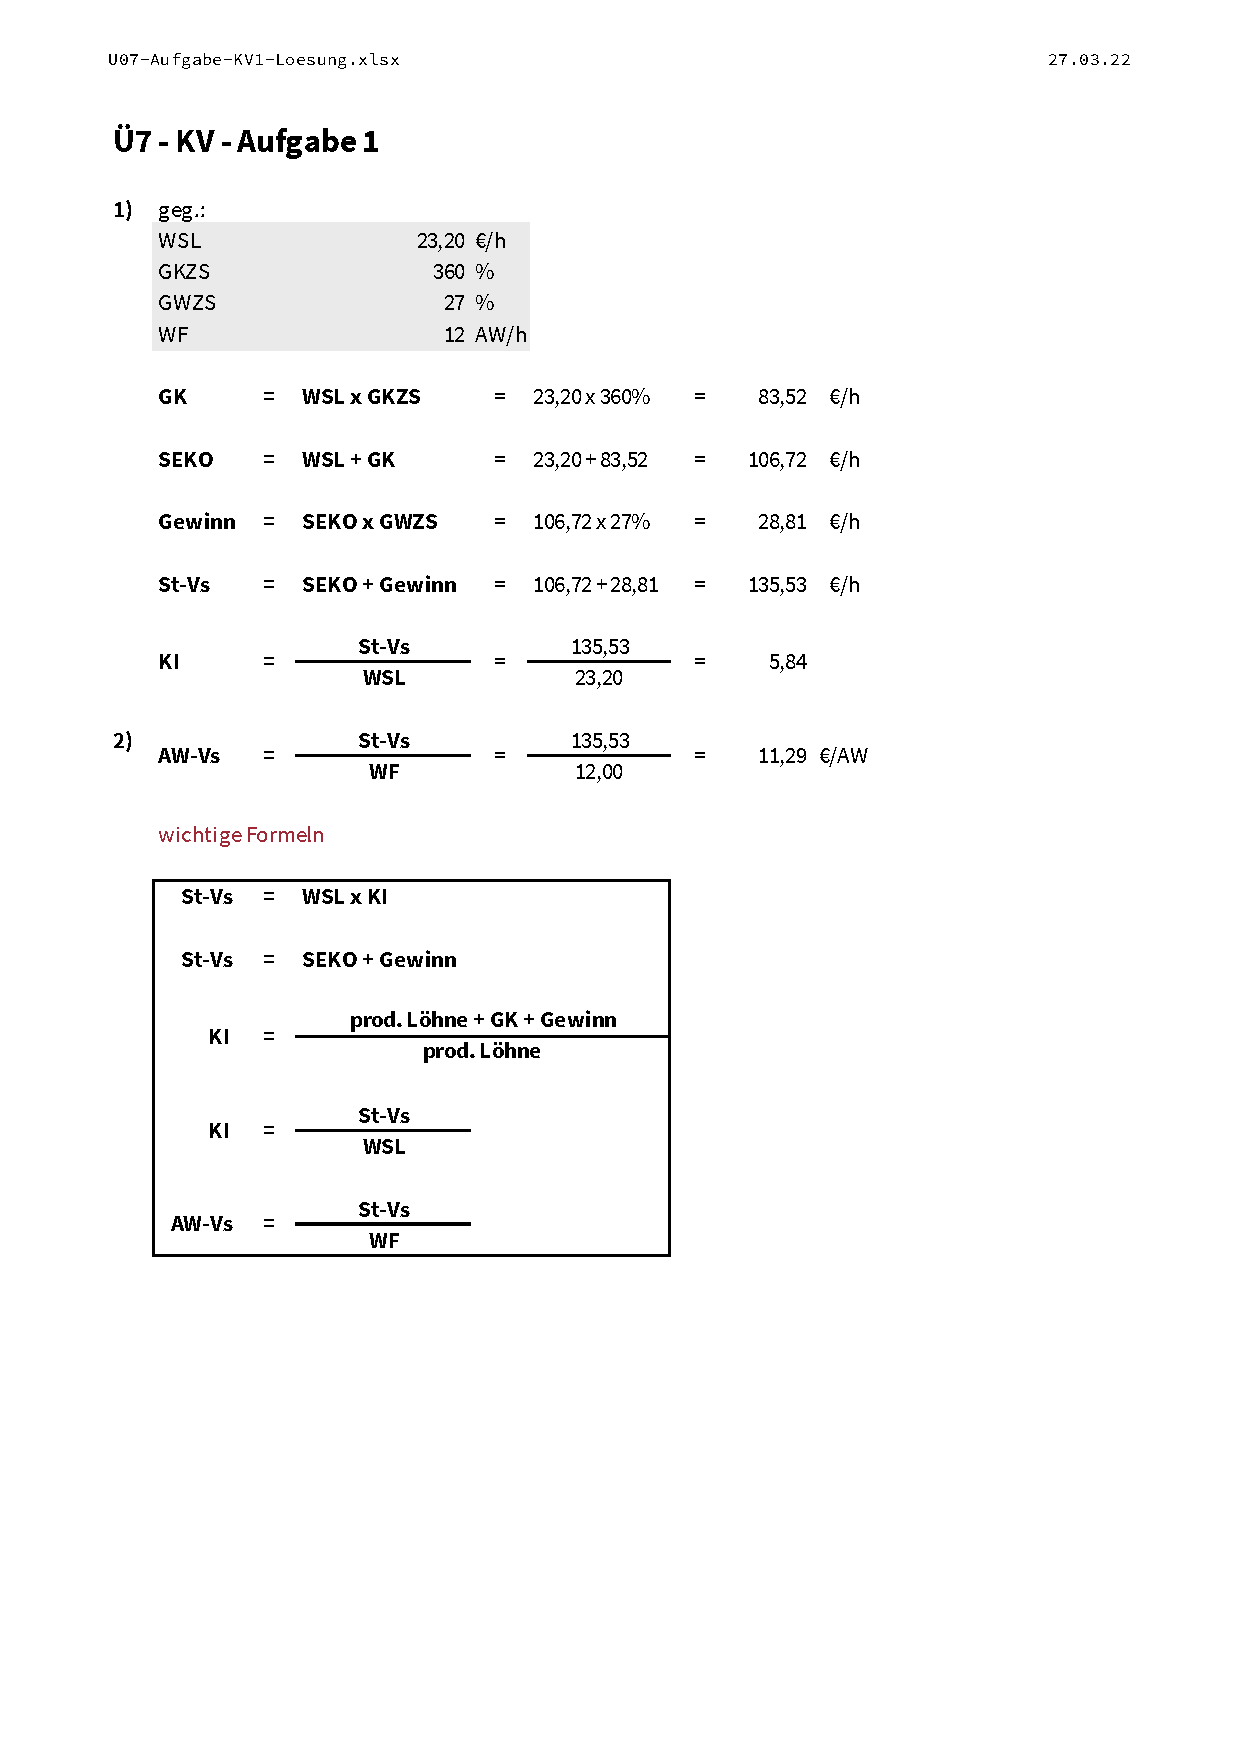
\includepdf[pages=-]{Tabellen/PDF/U07-Aufgabe-KV1-Loesung.pdf}

% -------
\section{U08 - Aufgabe - KV2 - HFM}\label{sec:U08-Aufgabe-KV2-HFM}\index{U08-Aufgabe-KV2-HFM}
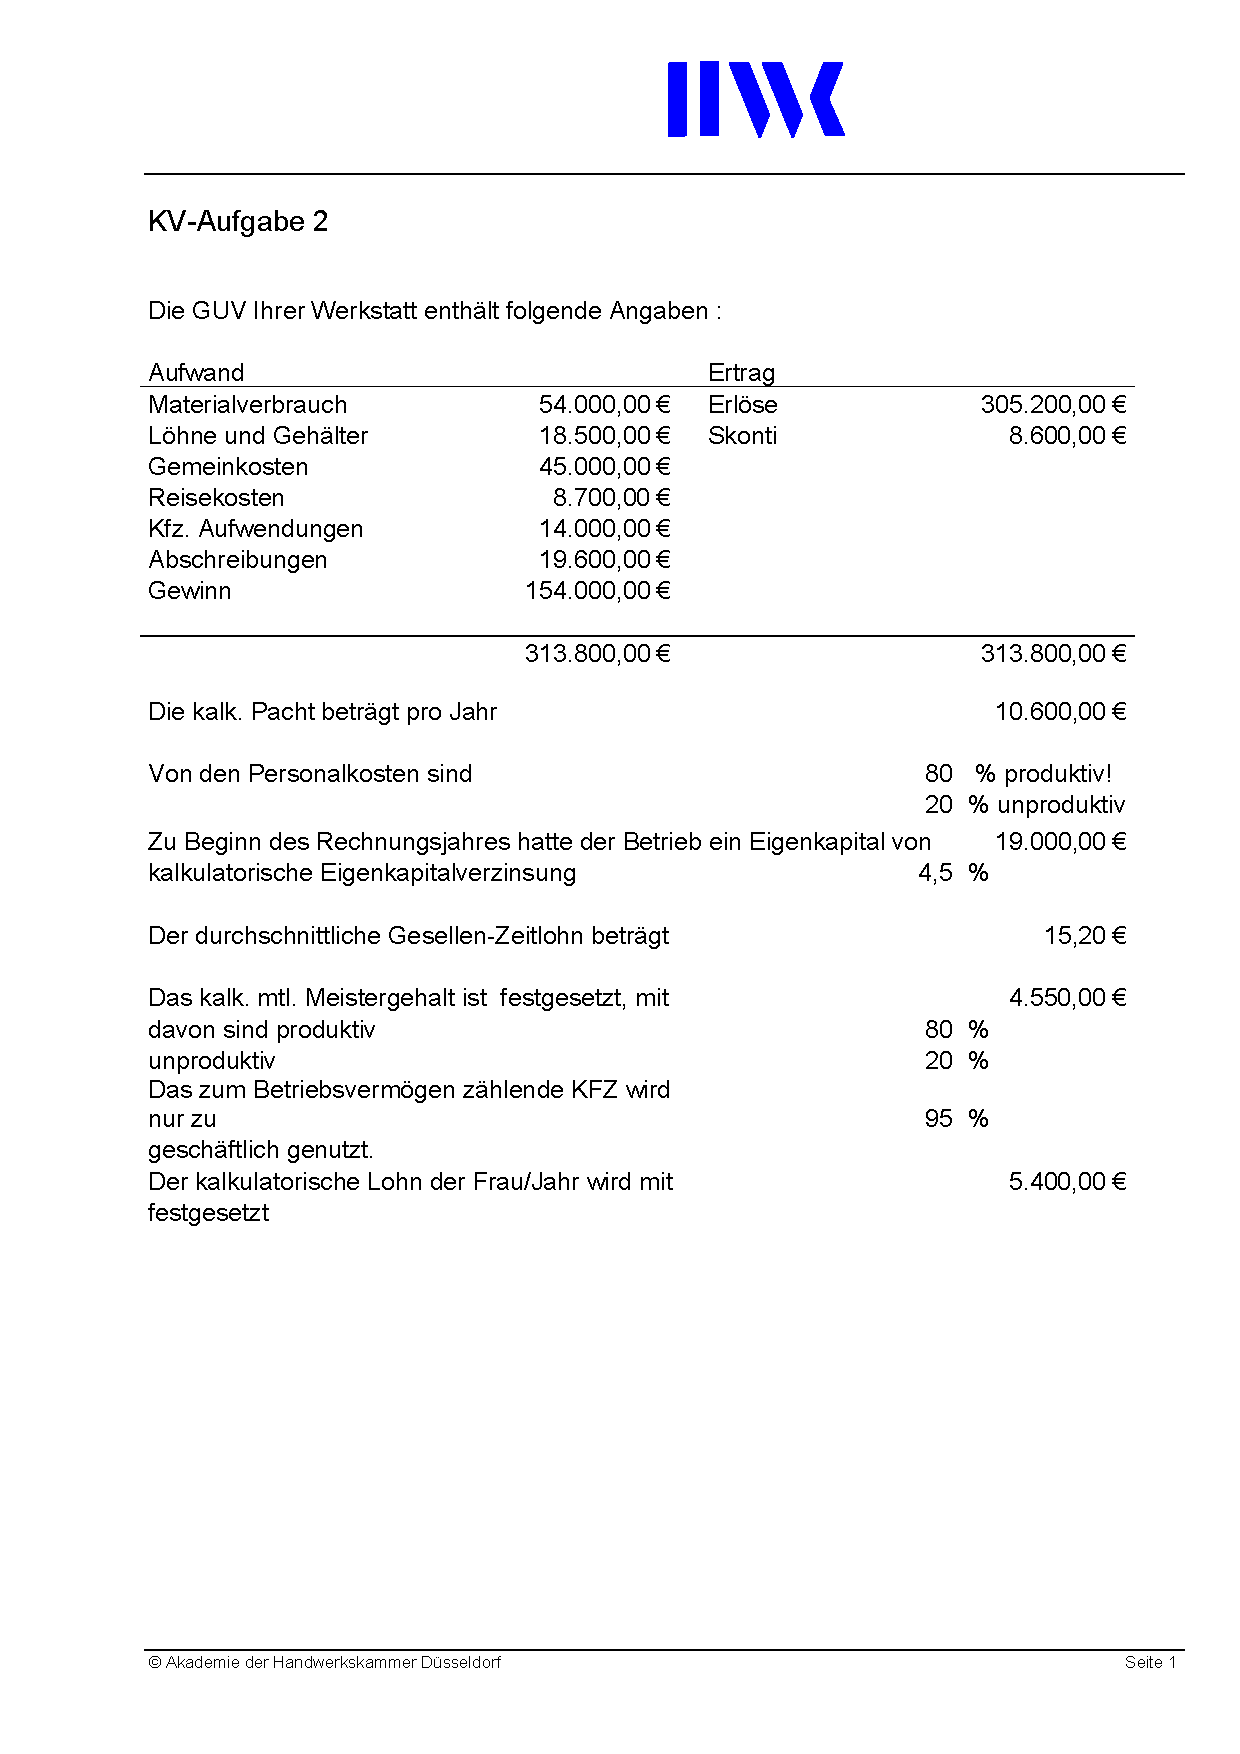
\includepdf[pages=-]{Tabellen/PDF/U08-Aufgabe-KV2-HFM.pdf}
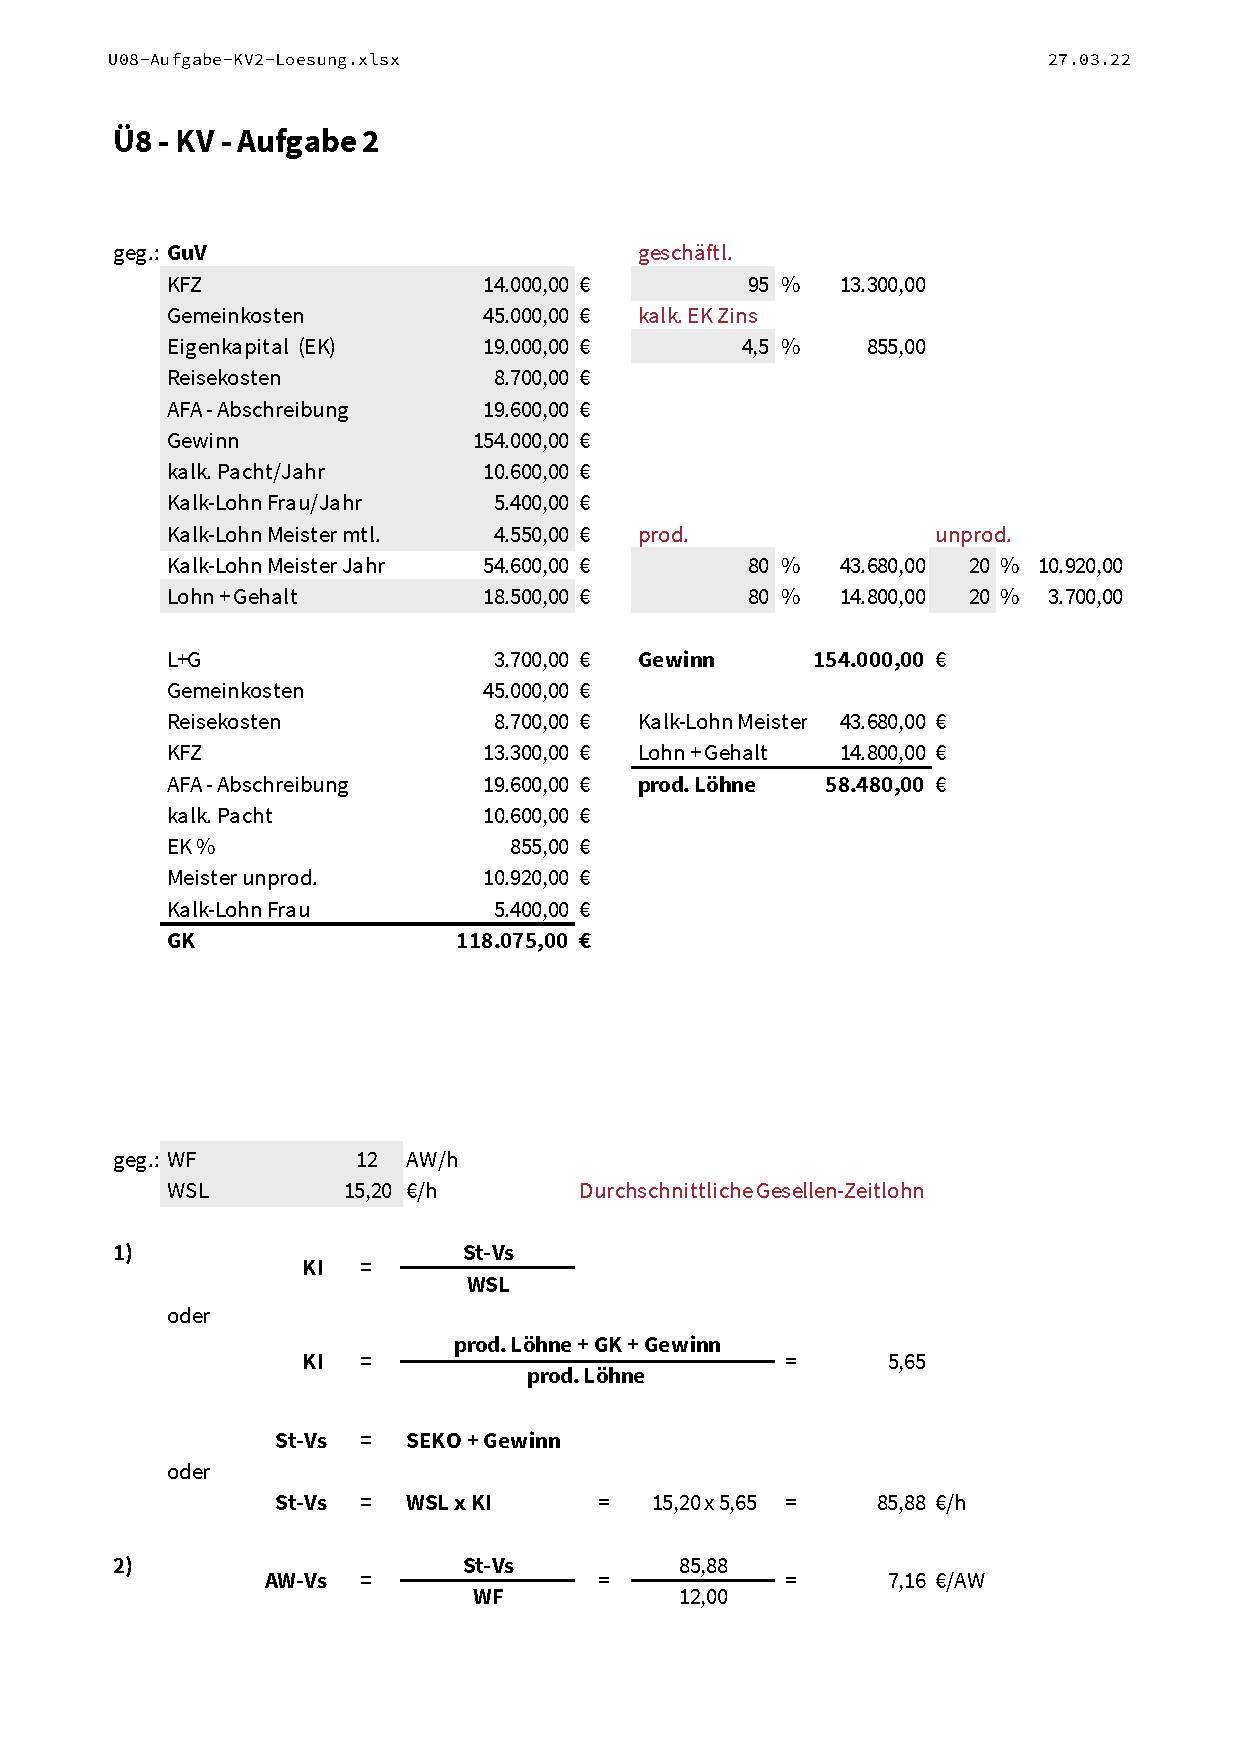
\includepdf[pages=-]{Tabellen/PDF/U08-Aufgabe-KV2-Loesung.pdf}

% -------
\section{U09 - Aufgabe - KV3}\label{sec:U09-Aufgabe-KV3}\index{U09-Aufgabe-KV3}
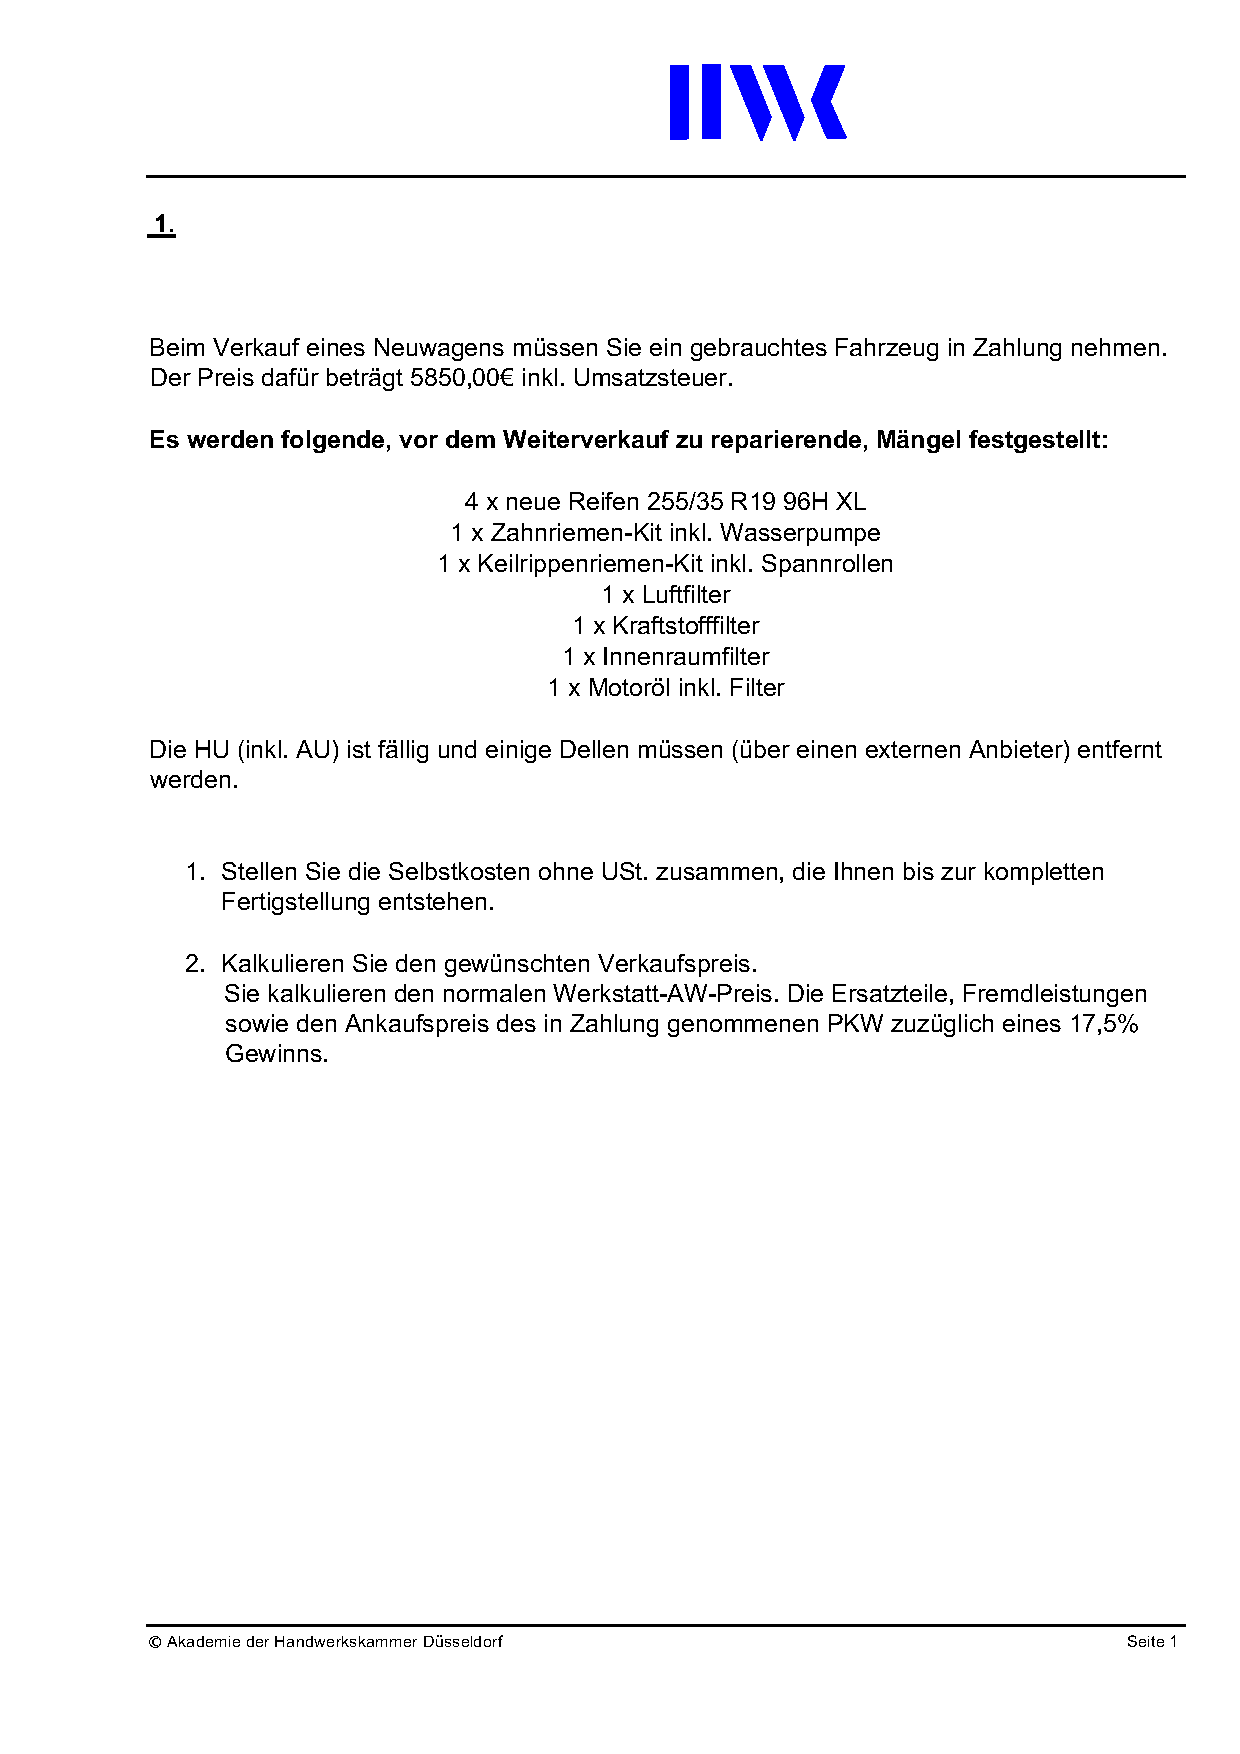
\includepdf[pages=-]{Tabellen/PDF/U09-Aufgabe-KV3.pdf}
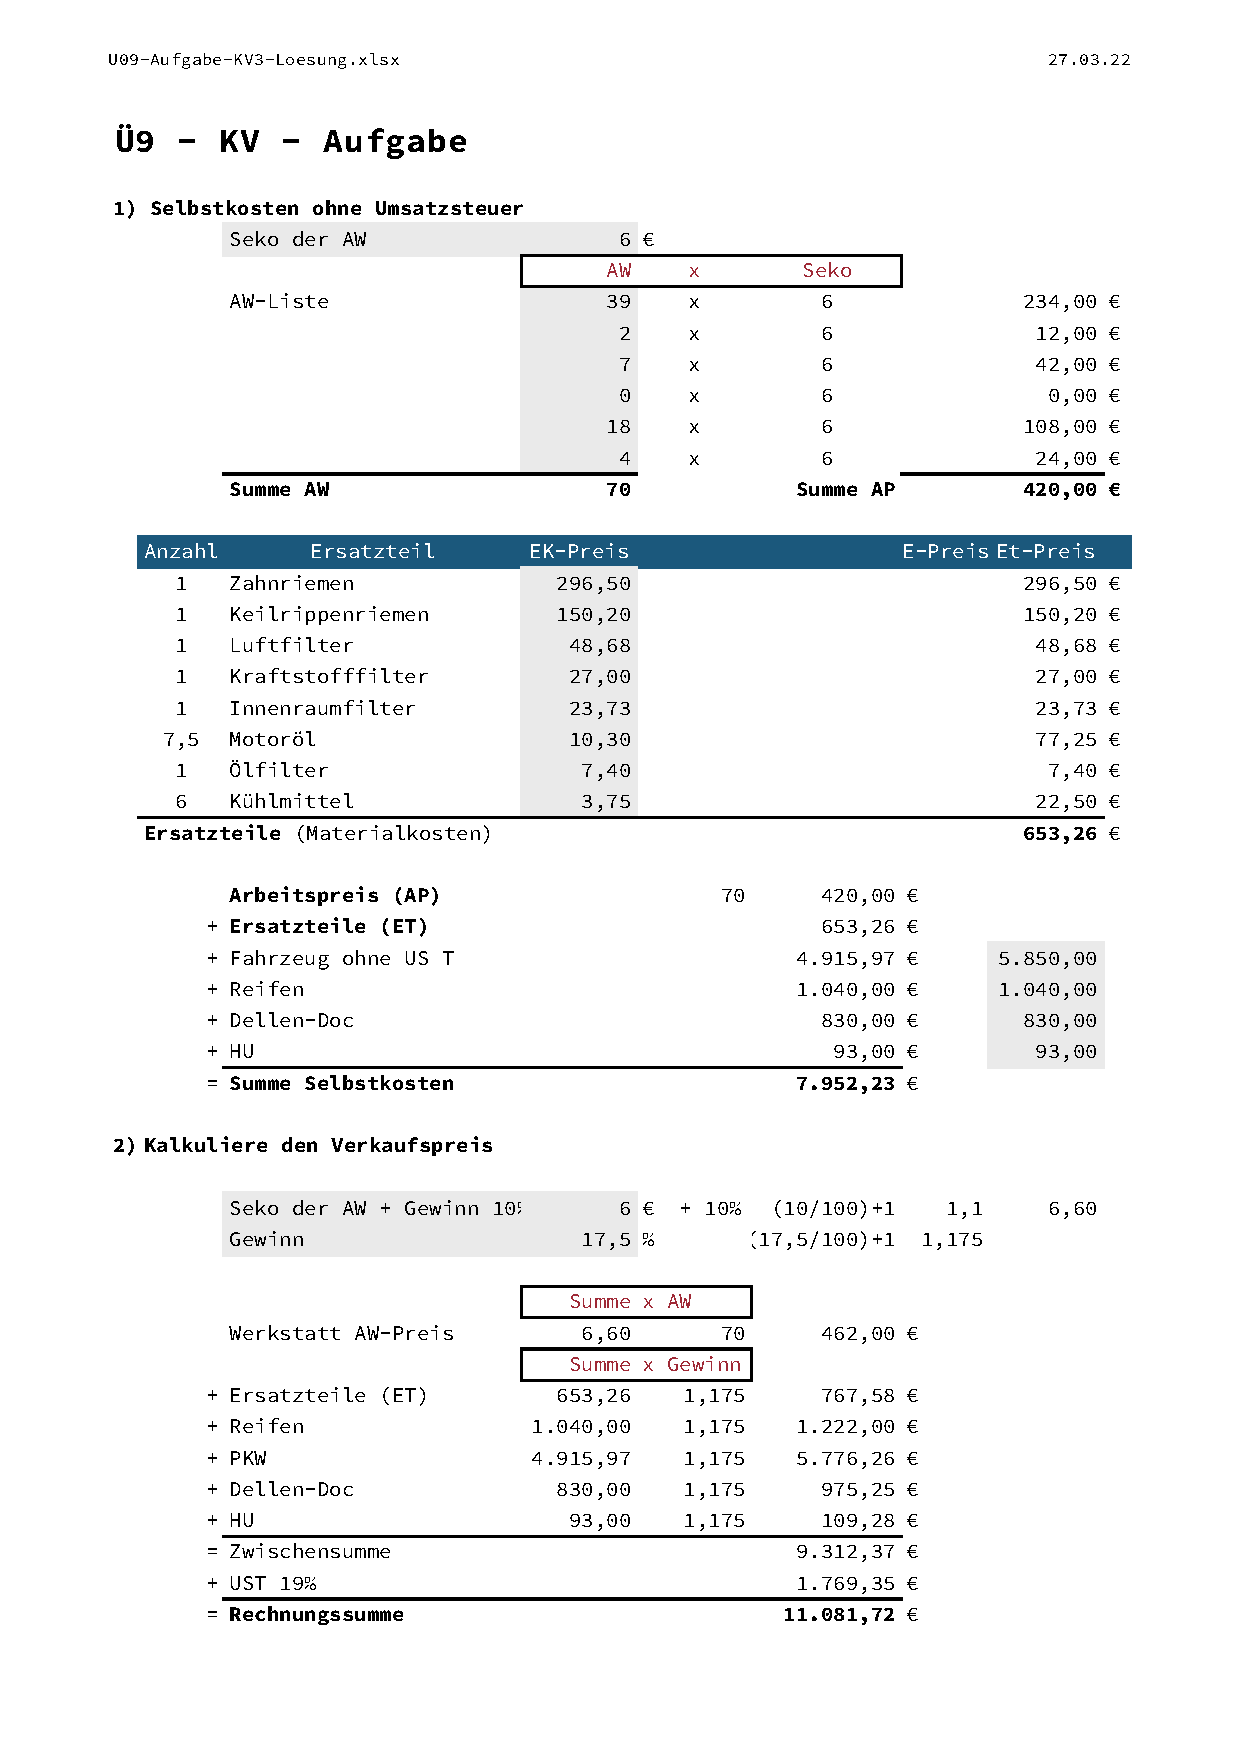
\includepdf[pages=-]{Tabellen/PDF/U09-Aufgabe-KV3-Loesung.pdf}

% -------
\section{U10 - Prüfungsaufgabentraining}\label{sec:U10-Pruefungsaufgabentraining}\index{U10-Pruefungsaufgabentraining}
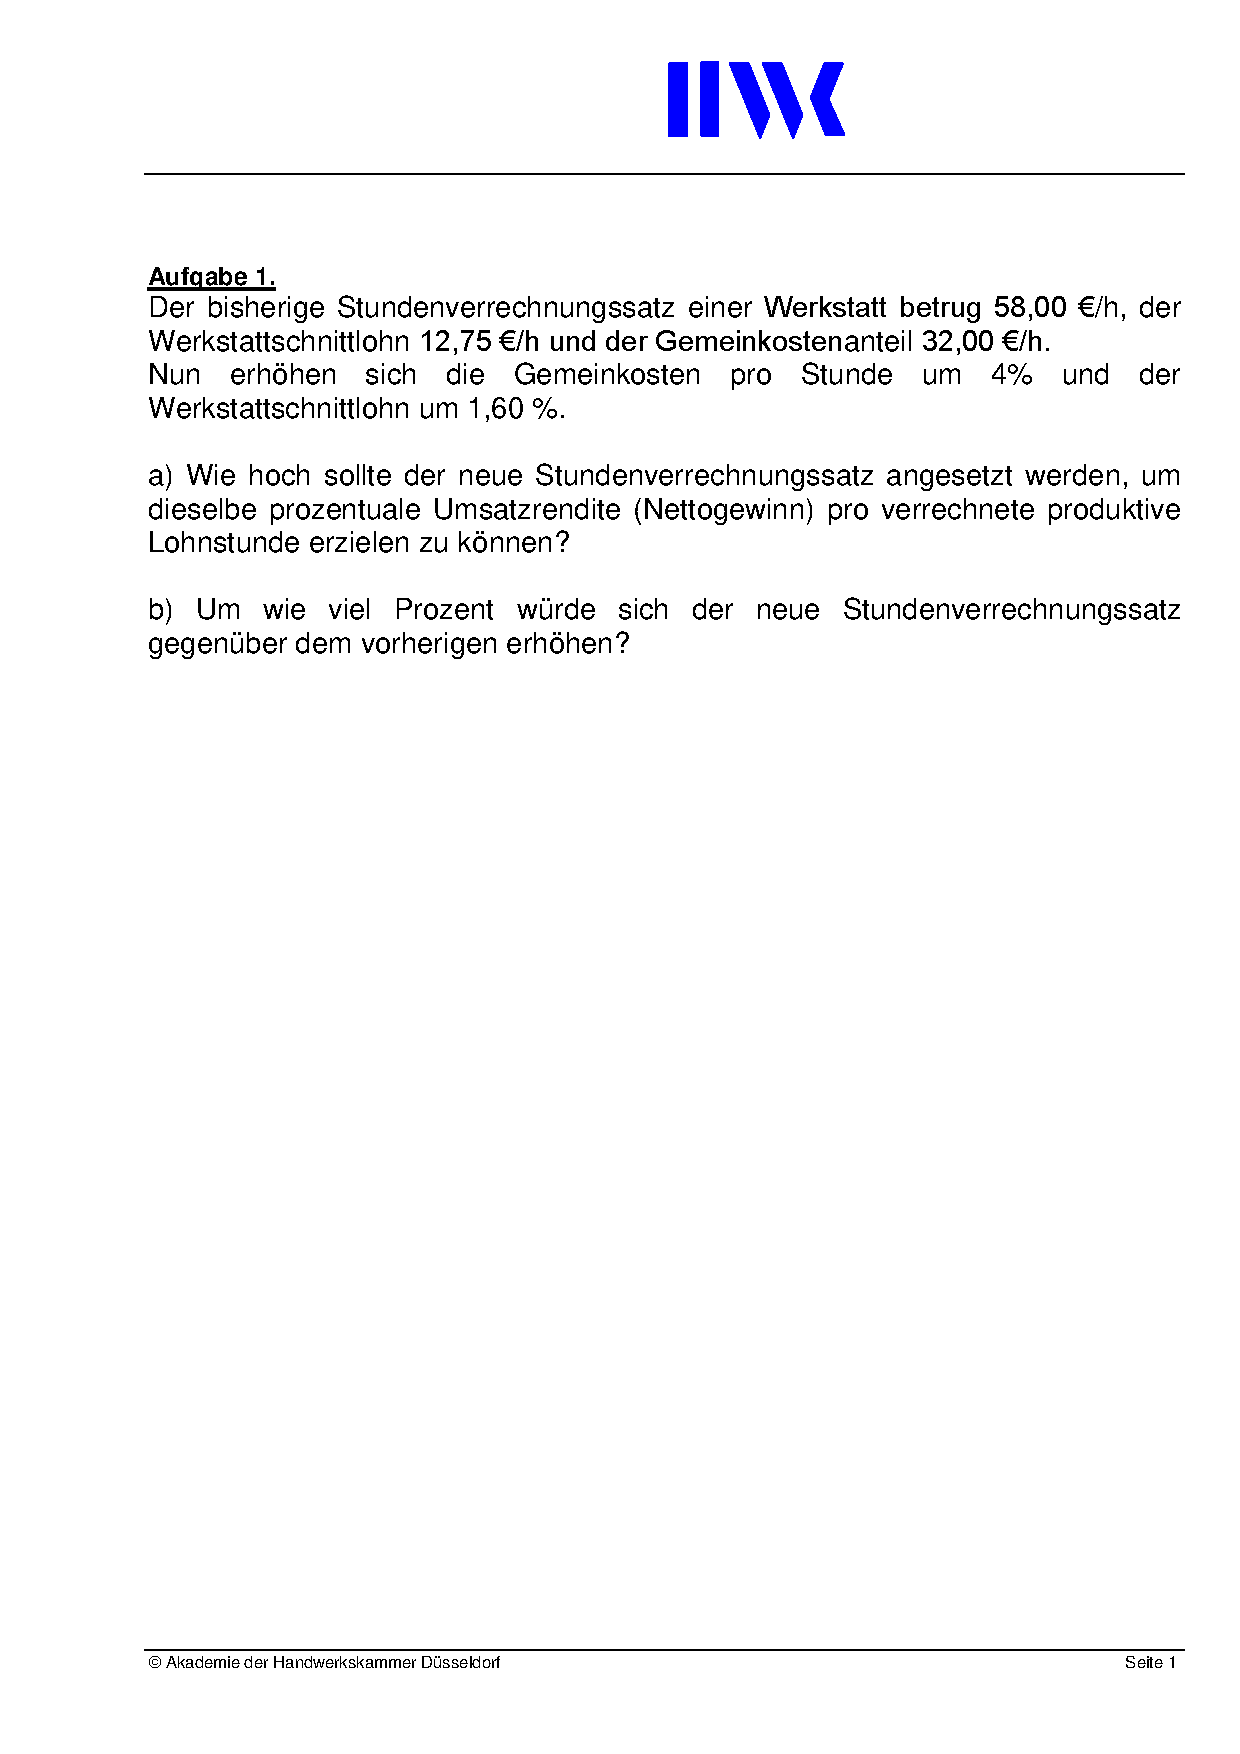
\includepdf[pages=-]{Tabellen/PDF/U10-Pruefungsaufgabentraining.pdf}
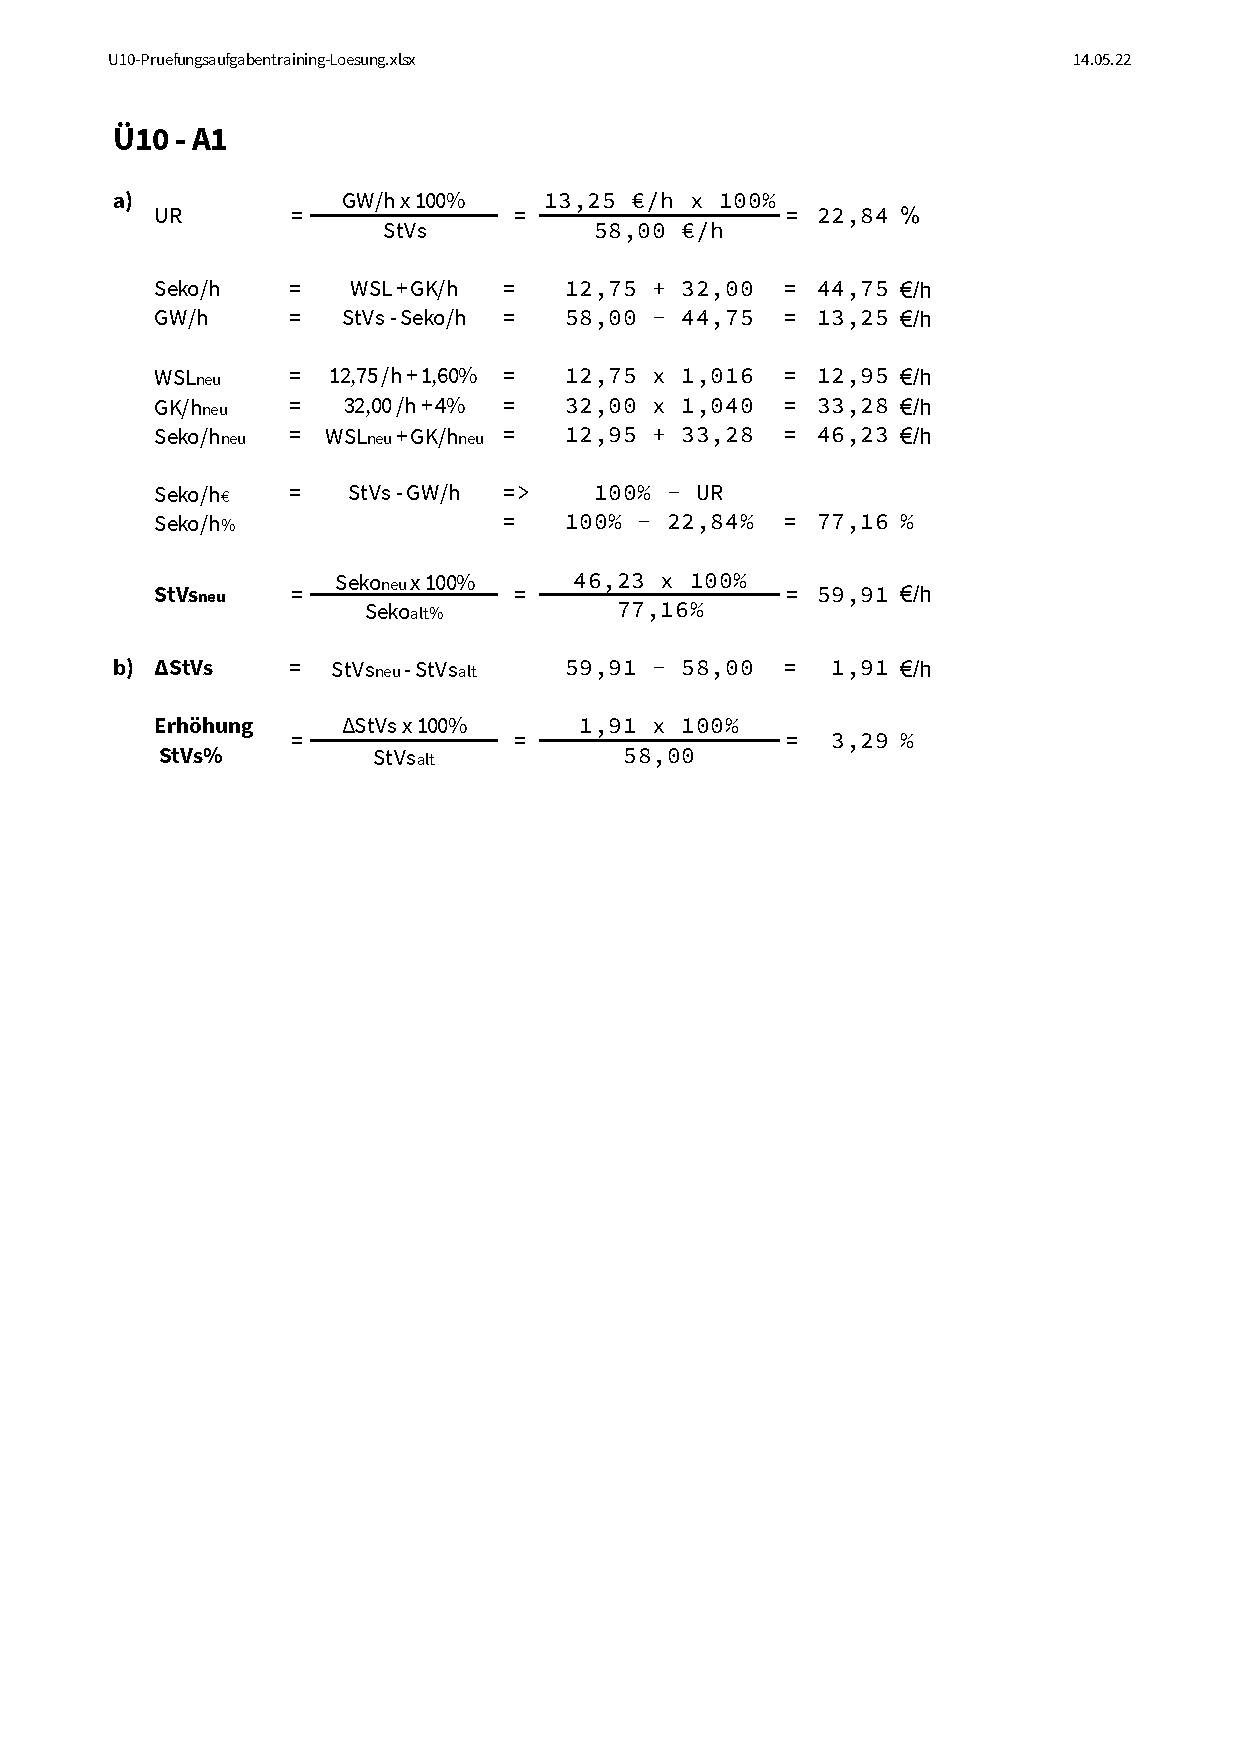
\includepdf[pages=-]{Tabellen/PDF/U10-Pruefungsaufgabentraining-Loesung.pdf}

% -------
\section{U11 - Aufgabe - Afa}

siehe Script

% -------
\section{U12 - Aufgabe - Leistungslohnsatz}\label{sec:U12-Aufgabe-Leistungslohnsatz}\index{U12-Aufgabe-Leistungslohnsatz}
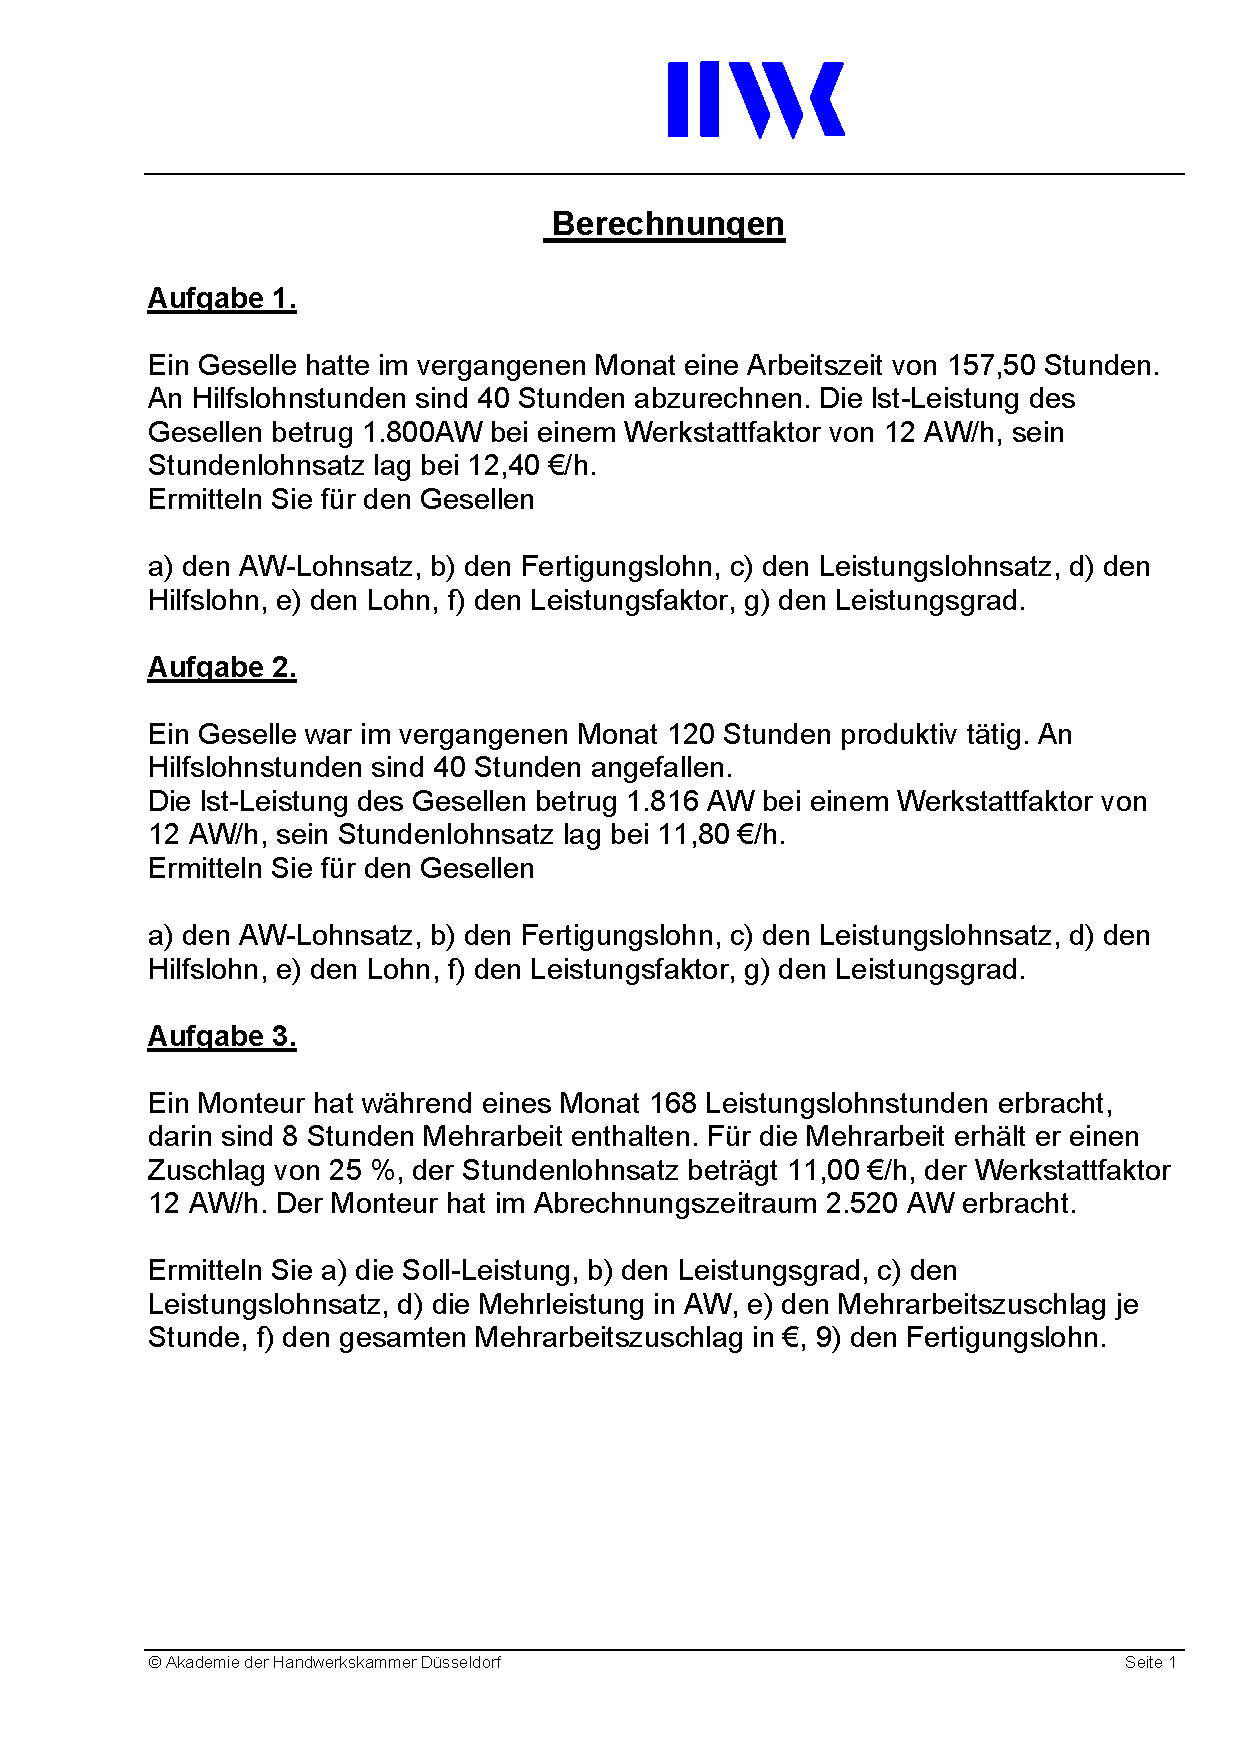
\includepdf[pages=-]{Tabellen/PDF/U12-Aufgabe-Leistungslohnsatz.pdf}
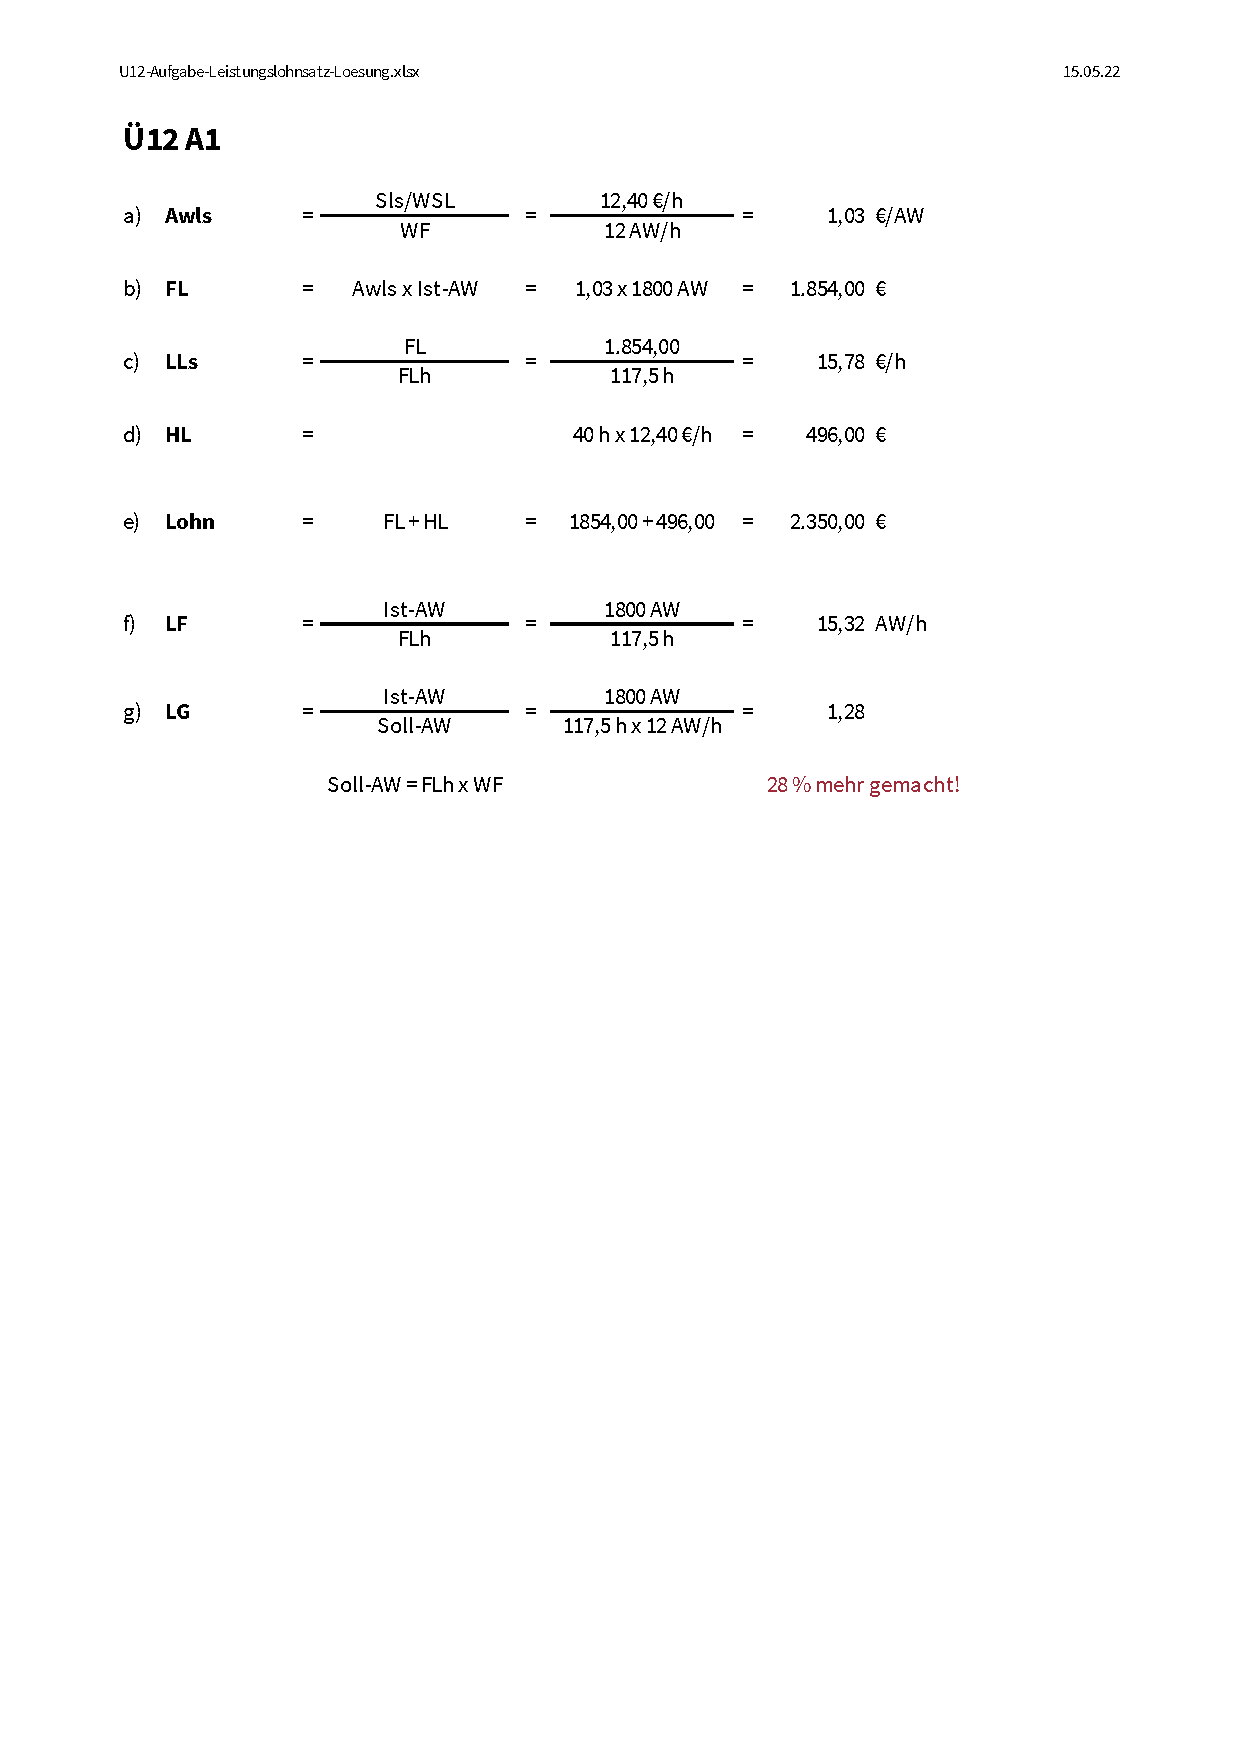
\includepdf[pages=-]{Tabellen/PDF/U12-Aufgabe-Leistungslohnsatz-Loesung.pdf}

% -------
\section{U13 - Kundenblätter - test Lösung}\label{sec:U13-Kundenblaetter-test-Loesung}\index{U13-Kundenblaetter-test-Loesung}
%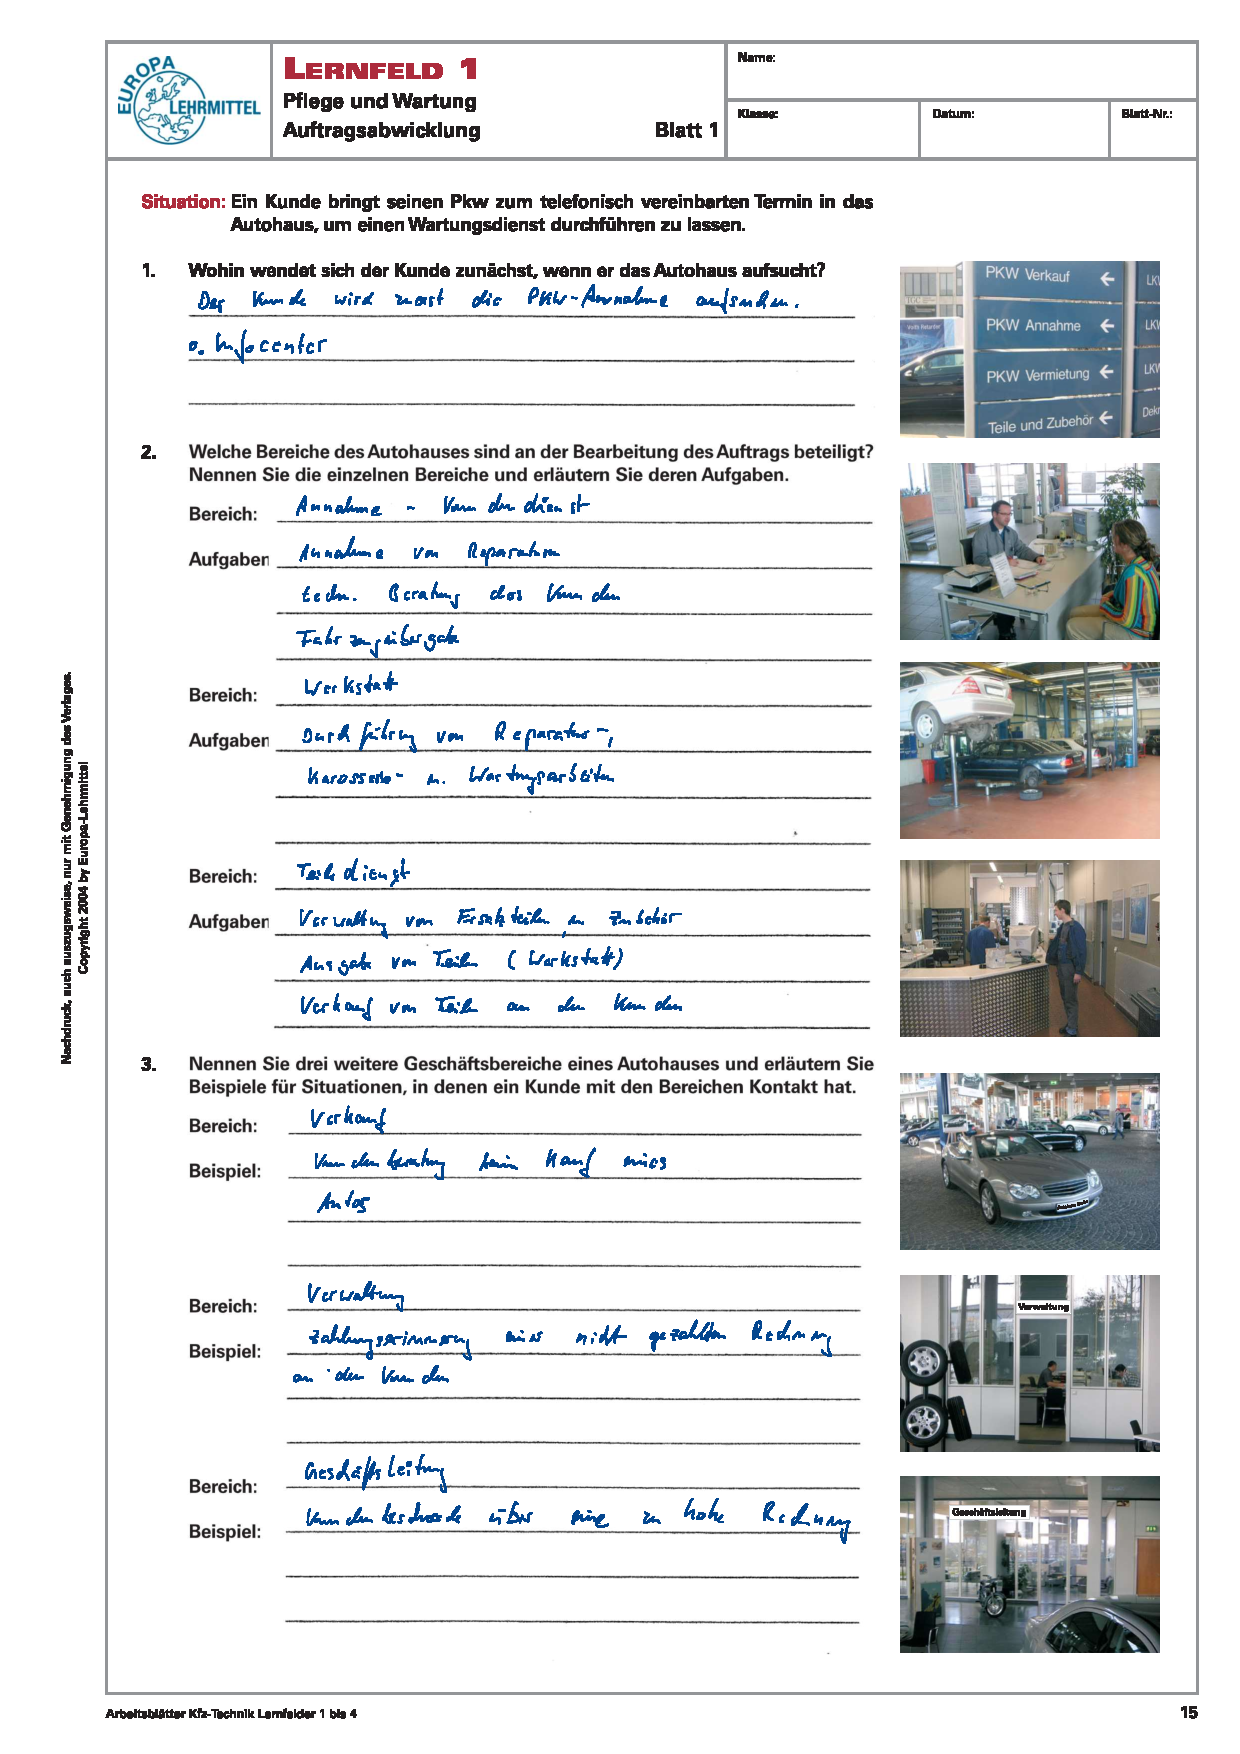
\includepdf[pages=-]{Tabellen/PDF/U13-Kundenblaetter-test-Loesung.pdf}

siehe Script








	%\input{content/tex/.tex}

    % Bibliographie
    \printbibliography
\end{document}
